\documentclass{beamer}
\documentclass[handout]{beamer}

\mode<handout>
{
  \usepackage{pgf}
  \usepackage{pgfpages}

\pgfpagesdeclarelayout{4 on 1 boxed}
{
  \edef\pgfpageoptionheight{\the\paperheight} 
  \edef\pgfpageoptionwidth{\the\paperwidth}
  \edef\pgfpageoptionborder{0pt}
}
{
  \pgfpagesphysicalpageoptions
  {%
    logical pages=4,%
    physical height=\pgfpageoptionheight,%
    physical width=\pgfpageoptionwidth%
  }
  \pgfpageslogicalpageoptions{1}
  {%
    border code=\pgfsetlinewidth{2pt}\pgfstroke,%
    border shrink=\pgfpageoptionborder,%
    resized width=.5\pgfphysicalwidth,%
    resized height=.5\pgfphysicalheight,%
    center=\pgfpoint{.25\pgfphysicalwidth}{.75\pgfphysicalheight}%
  }%
  \pgfpageslogicalpageoptions{2}
  {%
    border code=\pgfsetlinewidth{2pt}\pgfstroke,%
    border shrink=\pgfpageoptionborder,%
    resized width=.5\pgfphysicalwidth,%
    resized height=.5\pgfphysicalheight,%
    center=\pgfpoint{.75\pgfphysicalwidth}{.75\pgfphysicalheight}%
  }%
  \pgfpageslogicalpageoptions{3}
  {%
    border code=\pgfsetlinewidth{2pt}\pgfstroke,%
    border shrink=\pgfpageoptionborder,%
    resized width=.5\pgfphysicalwidth,%
    resized height=.5\pgfphysicalheight,%
    center=\pgfpoint{.25\pgfphysicalwidth}{.25\pgfphysicalheight}%
  }%
  \pgfpageslogicalpageoptions{4}
  {%
    border code=\pgfsetlinewidth{2pt}\pgfstroke,%
    border shrink=\pgfpageoptionborder,%
    resized width=.5\pgfphysicalwidth,%
    resized height=.5\pgfphysicalheight,%
    center=\pgfpoint{.75\pgfphysicalwidth}{.25\pgfphysicalheight}%
  }%
}


  \pgfpagesuselayout{4 on 1 boxed}[a4paper, border shrink=5mm, landscape]
  \nofiles
}
 % for handout 
%\setbeameroption{show notes} % uncomment to the the notes

\usepackage[T2A]{fontenc}
\usepackage[utf8]{inputenc}
\usepackage[russian]{babel}
\usepackage{amssymb,amsfonts,amsmath,mathtext}
\usepackage{cite,enumerate,float,indentfirst}
\usepackage[dvips]{graphicx}
\usepackage[linesnumbered,ruled,vlined]{algorithm2e} % NEW
\usepackage{algorithmic}

%\usepackage{graphicx,amssymb,amstext,amsmath,amsthm}
%\usepackage{mathrsfs}

\usepackage{listings}

\lstset{
        breaklines=true,
        basicstyle=\footnotesize\ttfamily,
        prebreak =\raisebox{0ex}[0ex][0ex]{\ensuremath{\hookleftarrow}},
        postbreak =\raisebox{0ex}[0ex][0ex]{\ensuremath{\hookleftarrow}}
}

\setbeamertemplate{footline}[page number]

\title[\insertframenumber/\inserttotalframenumber]
{\textbf{Вычислительная лексическая семантика: метрики семантической близости и их приложения}}

\subtitle{НИУ ВШЭ}

\author[Александр Панченко]
{\textbf{Александр Панченко} \\ Digital Society Laboratory \& Université
catholique de Louvain
\\
{
\url{alexander.panchenko@uclouvain.be}  }}
%\date{}

%\author[Александр Панченко]
%{\textbf{Александр Панченко} \\ Digital Society Laboratory \& Université catholique de Louvain
%\\
%	{
%	 \url{alexander.panchenko uclouvain.be} 
%	  }
%}


 %\\ Серия лекций в НИУ ВШЭ, факультет бизнес-информатики и прикладной математики (Нижний Новгород)

\mode<presentation>
{
%\usetheme{Warsaw} % default beamer
%\usetheme{Singapore} % plain white
\usetheme{Luebeck}
\usecolortheme{default}
%\usecolortheme{orchid}% plain white
\useoutertheme{smoothbars}
%\usefonttheme{serif}
}


\setbeamertemplate{navigation symbols}{%
}

\AtBeginSubsection[]
{
	\begin{frame}<beamer>
  	\frametitle{План}
  	\tableofcontents[currentsection,currentsubsection,currentsubsubsection]
  	\end{frame}
}


\AtBeginSection[]
{
	\begin{frame}<beamer>
	\frametitle{План}
	\tableofcontents[currentsection]
	\end{frame}
}

\begin{document}

\frame{ \titlepage \vspace{-0.7cm}
   \begin{center}
    
\includegraphics[width=.22\textwidth]{figures/dsl}
    \includegraphics[width=.15\textwidth]{figures/ucl} 
    
    \end{center}
}


\begin{frame}
  \setcounter{tocdepth}{2}
  \frametitle{План}
  \tableofcontents
  \setcounter{tocdepth}{2}
	
\end{frame}


%%%%%%%%%%%%%%%%%%%%%%%%%%%%%%%%%%%%%%%%%%%%%%
% BEGIN
%%%%%%%%%%%%%%%%%%%%%%%%%%%%%%%%%%%%%%%%%%%%%%


\section[Lexical Semantics]{Computational Lexical Semanitcs}
\subsection{ }



\begin{frame}
\frametitle{Motivation}


\begin{figure}
\centering
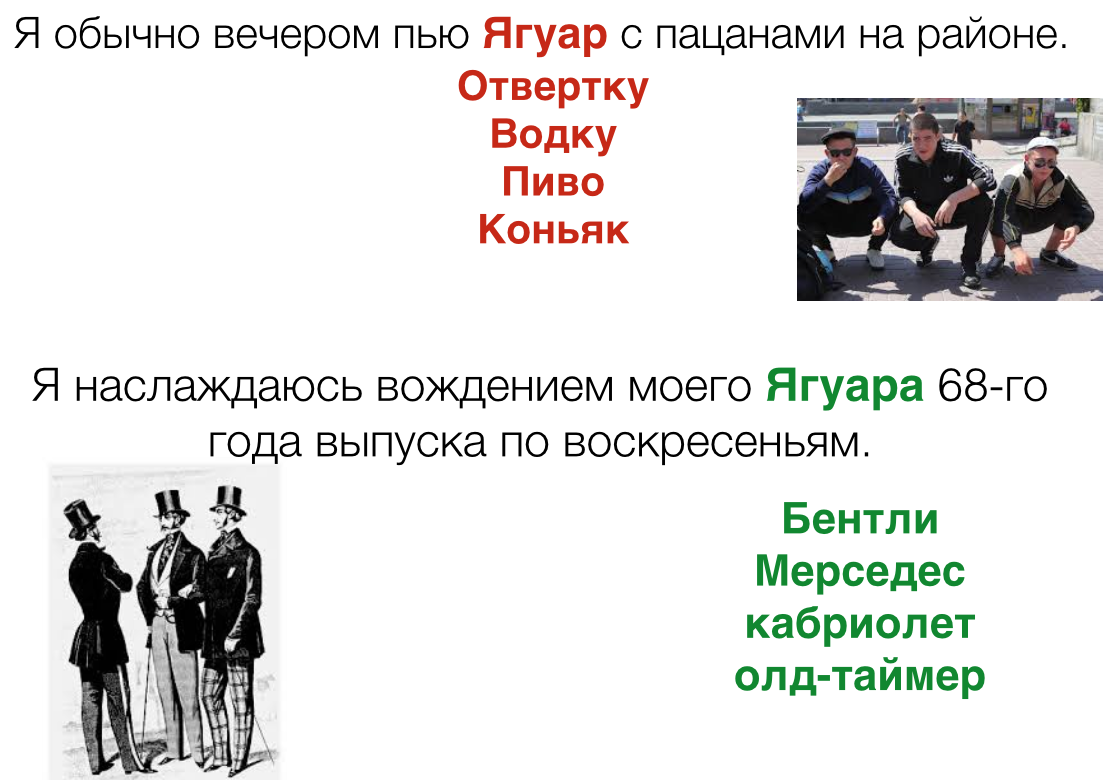
\includegraphics[width=0.95\textwidth]{./figures/jaguar}
\end{figure} 
\end{frame}


\begin{frame}
\frametitle{Two Worlds of Computational Lexical Semantics}


\begin{figure}
\centering
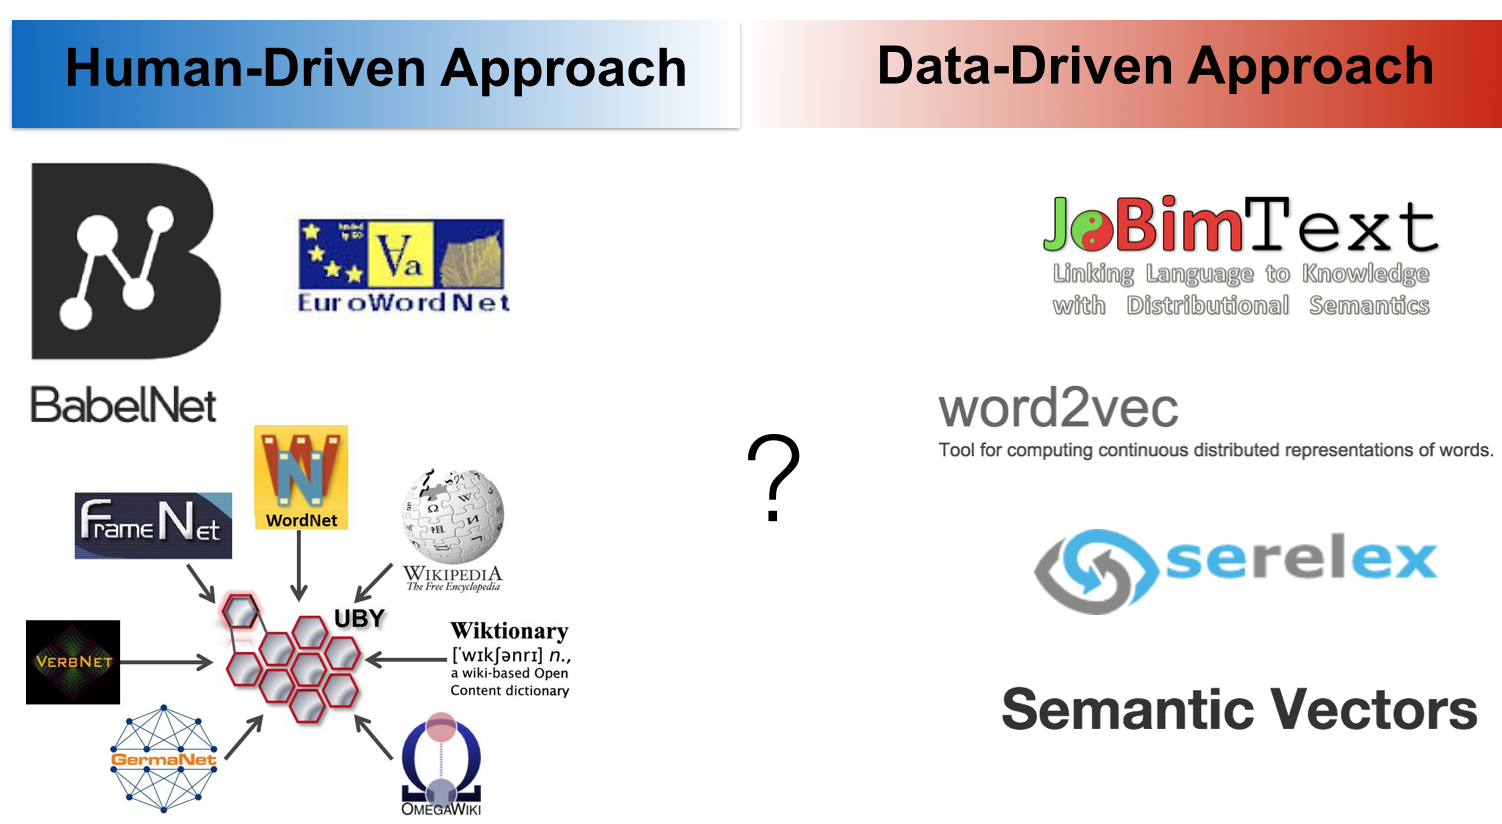
\includegraphics[width=1.0\textwidth]{./figures/two-worlds}
\end{figure} 
\end{frame}





\begin{frame}
\frametitle{Computational Lexical Semantics: Levels of Analysis}

\begin{figure}
\centering
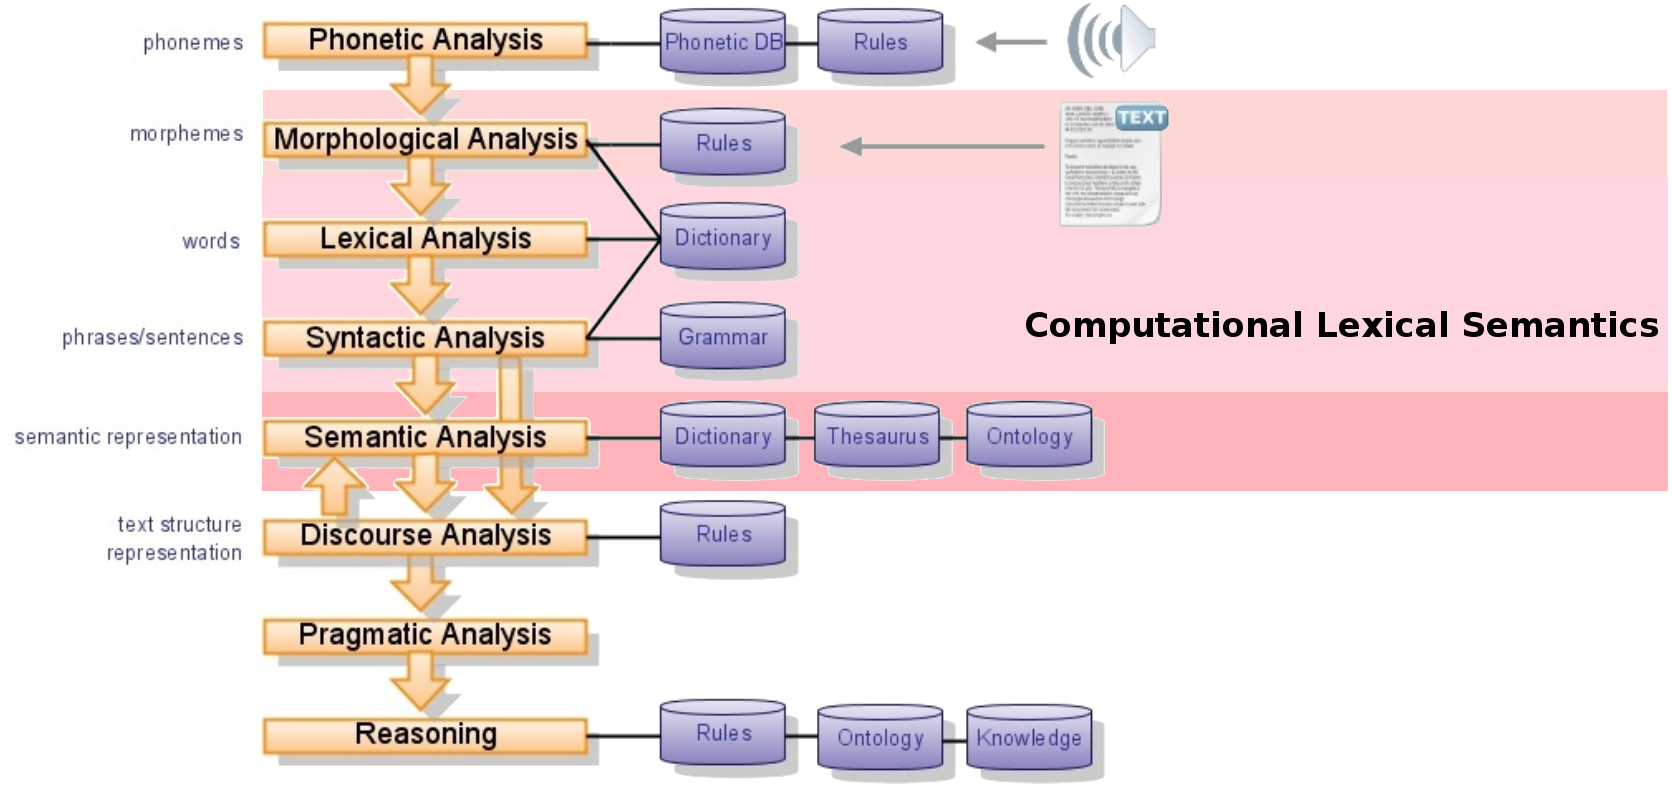
\includegraphics[width=1.05\textwidth]{figures/levels}
\end{figure}

 \tiny{* source of the image \url{http://www.uclouvain.be/en-cours-2013-LINGI2263.html}}

\end{frame}





\begin{frame}
\frametitle{Tasks}

\textbf{Computational models} of semantics of words and multiword expressions are used to solve following tasks:
 
\begin{itemize}
  \item Word sense disambiguation (WSD) and named entity disambiguation;
  \item Semantic relation extraction;
  \item Semantic similarity and semantic relatedness;
  \item Word sense induction (WSI) and discrimination;
  \item Generation of features for other NLP tasks.
\end{itemize}

\end{frame}




\begin{frame}
\frametitle{Introduction into the field}

\begin{itemize}
  \item Jurafsky D. and Martin J.H. An \textbf{Introduction to Natural Language Processing, Computational Linguistics, and Speech Recognition} (2009), chapters 19,20, 22.

\item Cruys T. \textbf{Mining for meaning: the extraction of lexico-semantic knowledge from text} (2010). PhD thesis. \url{http://dissertations.ub.rug.nl/faculties/arts/2010/t.van.de.cruys/} 

\item Panchenko A. \textbf{Similarity Measures for Semantic Relation Extraction} (2013) \url{http://cental.fltr.ucl.ac.be/team/~panchenko/thesis.pdf} 


\end{itemize}


\end{frame}



\begin{frame}
\frametitle{Key concepts}

\begin{itemize}
 \item \textbf{Lexical unit}: word, multiword expression (MWE), noun phrase (NP).
 \item \textbf{Vocabulary}: a set of words. 
 \item \textbf{Semantic relation}: defines a connection between lexical units. Relation can have a numerical weight and/or a type, such as synonymy, hypernymy, co-hyponymy or association. 
 \item \textbf{Semantic resource}: Vocabulary + a set of semantic relations. 
 \item \textbf{Distributional thesaurus}: a semantic resource without types. 
 \item \textbf{Semantic relatedness/similarity}: a numerical measure of word similarity.
 \item \textbf{Synset}: a group of mutual synonyms. 
 \item \textbf{Sense}: sense of a lexical item. 
 \item \textbf{Sense inventory:} a set of senses of a given vocabulary. 
\end{itemize}


\end{frame}



\begin{frame}
\frametitle{Semantic Resources}

\begin{block}{}

A \textbf{semantic resource} is an graph $(C, R)$:
\begin{itemize}
\item nodes $C$ represent \textbf{terms};
\item edges $R$ represent untyped \textbf{semantic relations}.
\end{itemize}

\end{block}

\begin{figure}
\centering
\includegraphics[height=0.400\textwidth]{./../figures/sr-29-example-crop2}
\end{figure}

\end{frame}




\begin{frame}
\frametitle{Semantic Relations}
\begin{figure}
\centering
\includegraphics[width=0.65\textwidth]{./../figures/sr-29-example}
\caption{A semantic resource composed of 29 relations.}
\end{figure}

\end{frame}





\begin{frame}
\frametitle{Types of semantic relaitons}

\begin{figure}
\centering
\includegraphics[height=0.49\textwidth]{./../figures/sr-example-2}
\includegraphics[height=0.35\textwidth]{./../figures/sr-example-spacer}
\includegraphics[height=0.43\textwidth]{./../figures/sr-example-untyped-2}
\caption{A semantic resource with (a) typed (b) untyped relations. }
\end{figure}

\end{frame}



\begin{frame}
\frametitle{Types of semantic relations}

\begin{figure}
\centering
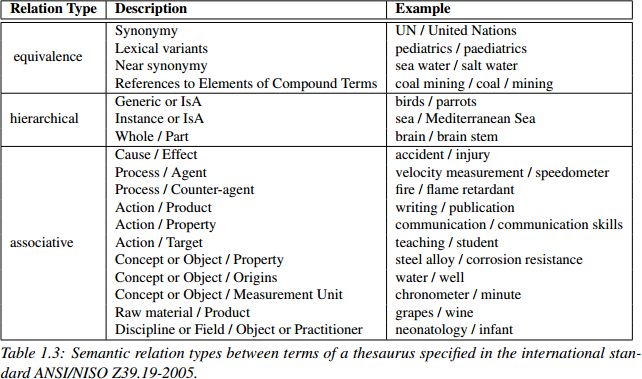
\includegraphics[height=0.49\textwidth]{./figures/sem-types}
\end{figure}

\end{frame}





\begin{frame}
\frametitle{Types of semantic relations}
\begin{figure}
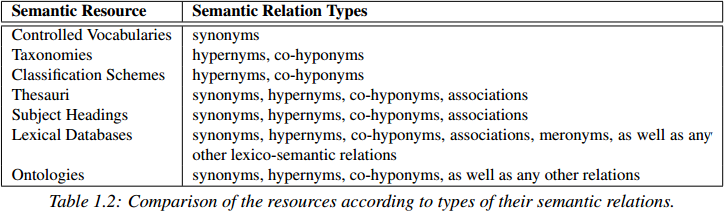
\includegraphics[width=1.0\textwidth]{figures/sem-res-table}
\end{figure}
\end{frame}







\frame{
\frametitle{Synsets}

\begin{figure}
\centering
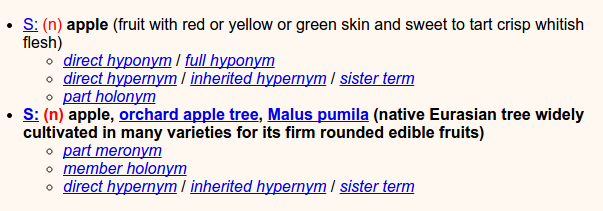
\includegraphics[width=0.9\textwidth]{figures/synset}
\caption{ WordNet synsets: \url{http://wordnetweb.princeton.edu/perl/webwn}. }
\end{figure}

}

\frame{
\frametitle{Synsets}

\begin{figure}
\centering
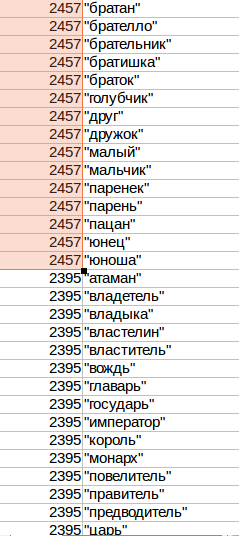
\includegraphics[width=0.26\textwidth]{figures/yarn}
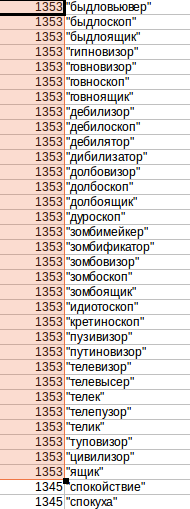
\includegraphics[width=0.22\textwidth]{figures/yarn2}
\caption{ YARN synsets: \url{http://russianword.net}. }
\end{figure}

}

\frame{
\frametitle{Synsets}

\begin{figure}
\centering
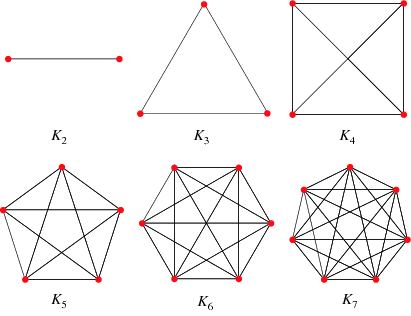
\includegraphics[width=0.7\textwidth]{figures/complete}
\caption{ Synset is a complete graph of synonyms. Source: \url{http://mathworld.wolfram.com/CompleteGraph.html}. }
\end{figure}

}

\begin{frame}
\frametitle{Semantic resources: expressiveness}

\begin{figure}
\centering
\includegraphics[width=0.9\textwidth]{../figures/expressivness}
\caption{ Expressiveness of different semantic resources. }
\label{fig:expressiveness}
\end{figure}

\end{frame}





\begin{frame}
\frametitle{Semantic resources: taxonomy }

\begin{figure}
\centering
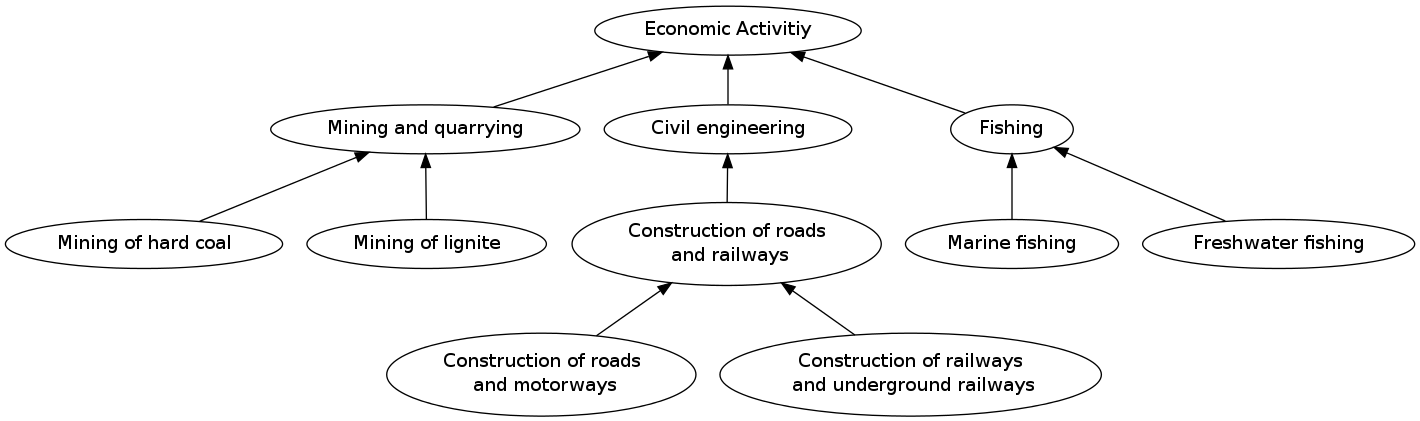
\includegraphics[width=1.0\textwidth]{figures/taxonomy-new}
\caption{ A part of the taxonomy of economical activities NACE.}
\label{fig:taxonomy}
\end{figure}

\end{frame}





\begin{frame}
\frametitle{Semantic resources: thesaurus }

\begin{figure}
\centering
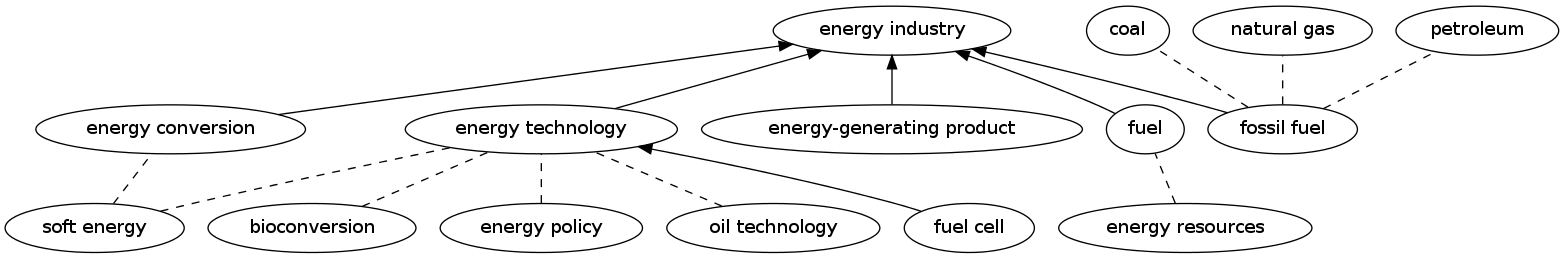
\includegraphics[width=1.0\textwidth]{figures/thesaurus-new}
\caption{ The Eurovoc thesaurus: the term ``energy industry'' and its semantic relations. Here, hypernyms are denoted with arrows and associations are denoted with dashed lines.}
\label{fig:thesaurus}
\end{figure}
\end{frame}




\begin{frame}
\frametitle{Semantic resources: lexical database }

\begin{figure}
\centering
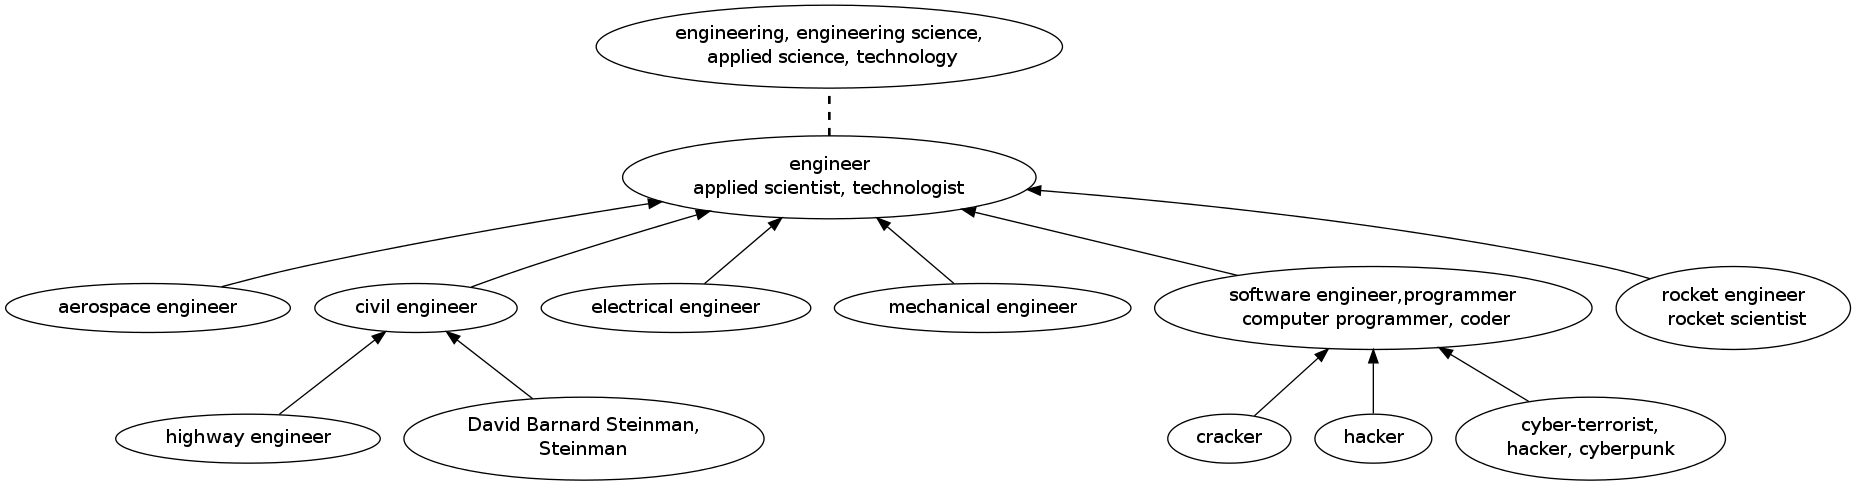
\includegraphics[width=1.0\textwidth]{figures/wordnet-new}
\caption{ Lexical database WordNet: synset \textit{engineer} and its semantic relations. }
\label{fig:wordnet}
\end{figure}
\end{frame}


\begin{frame}
\frametitle{Semantic resources: lexical database}

\begin{figure}
\centering
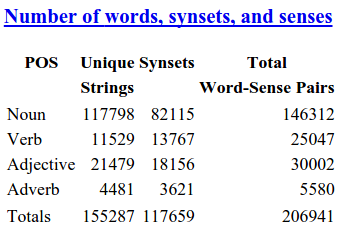
\includegraphics[width=.7\textwidth]{figures/wnstat}
\caption{ WordNet statistics. Source: \url{https://wordnet.princeton.edu/wordnet/man/wnstats.7WN.html} }
\label{fig:wordnet}
\end{figure}
\end{frame}



\begin{frame}
\frametitle{Semantic Resources: WordNet}

\begin{figure}
\centering
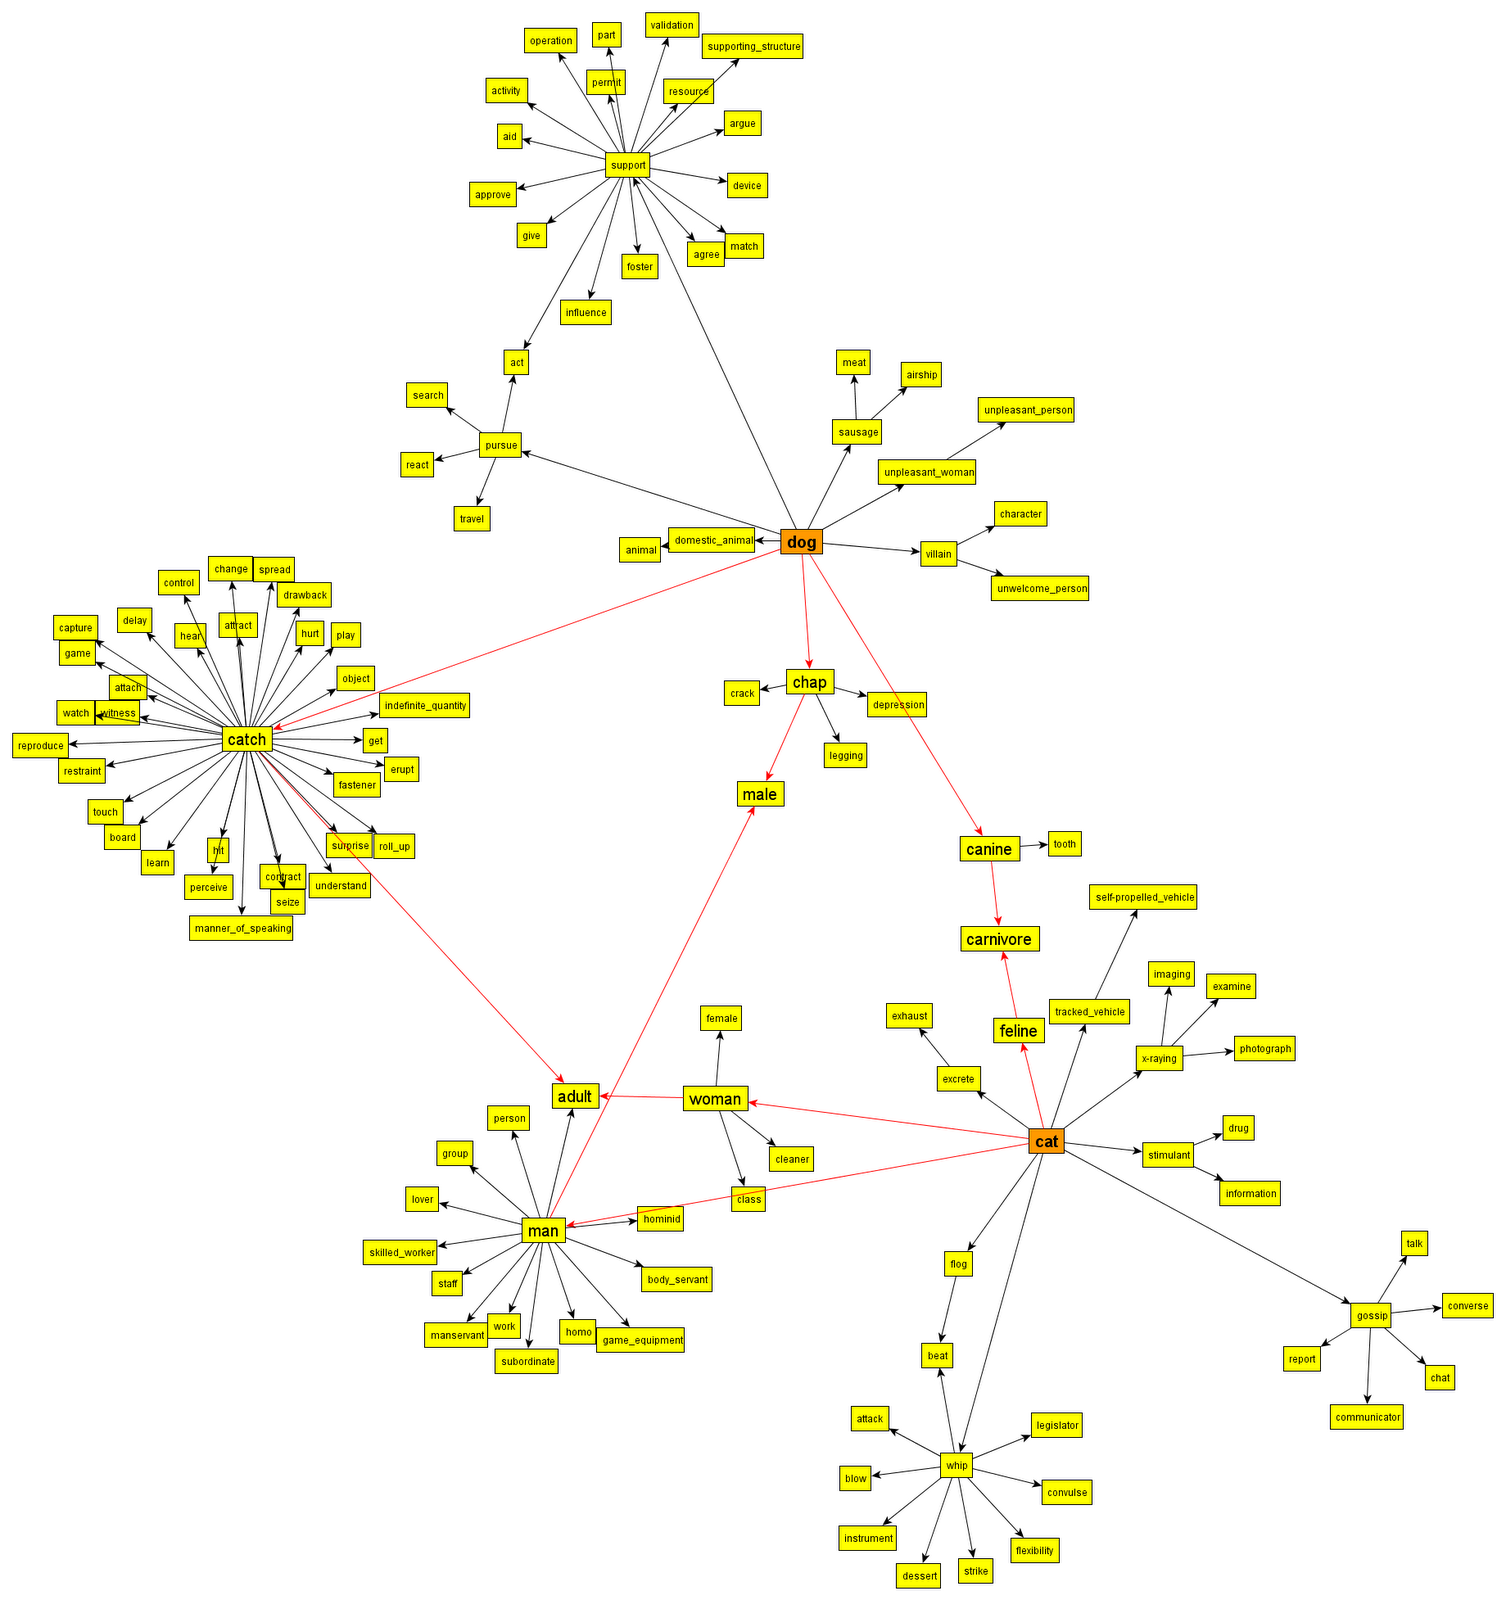
\includegraphics[width=0.65\textwidth]{figures/wordnet-big}
\label{fig:wordnet}
\end{figure}

{\footnotesize \url{http://geniferology.blogspot.com/2012/10/playing-with-wordnet.html}}
\end{frame}





\begin{frame}
\frametitle{A multilingual WordNet: BabelNet.org}

\begin{figure}
\centering
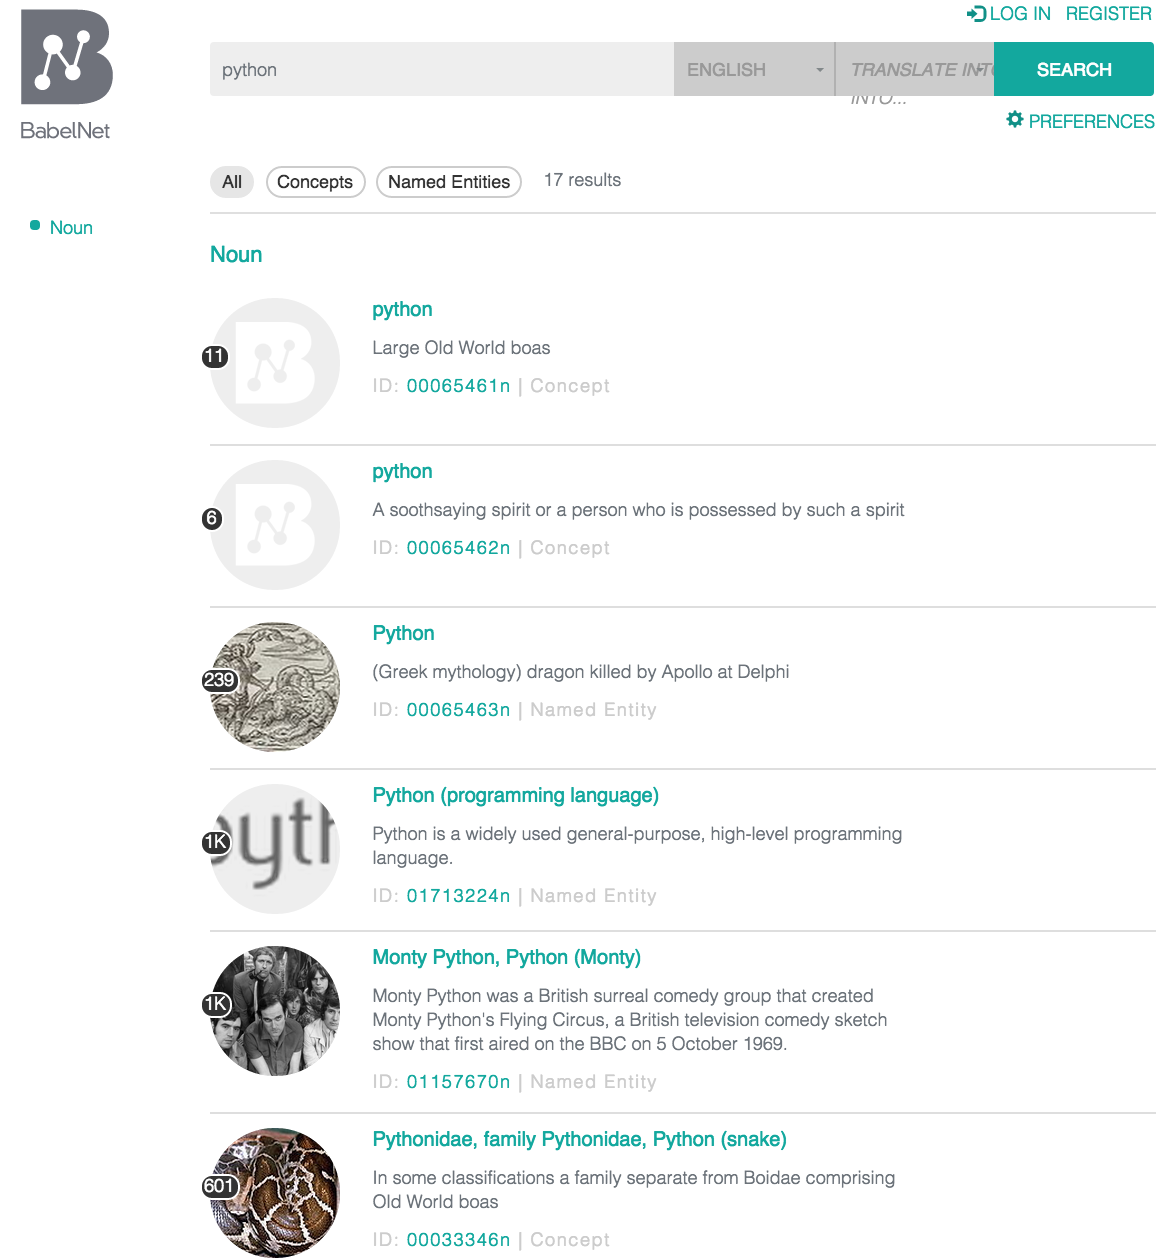
\includegraphics[height=0.7\textwidth]{./figures/babelnet1}
\end{figure}

\end{frame}




\begin{frame}
\frametitle{A multilingual WordNet: BabelNet.org}

\begin{figure}
\centering
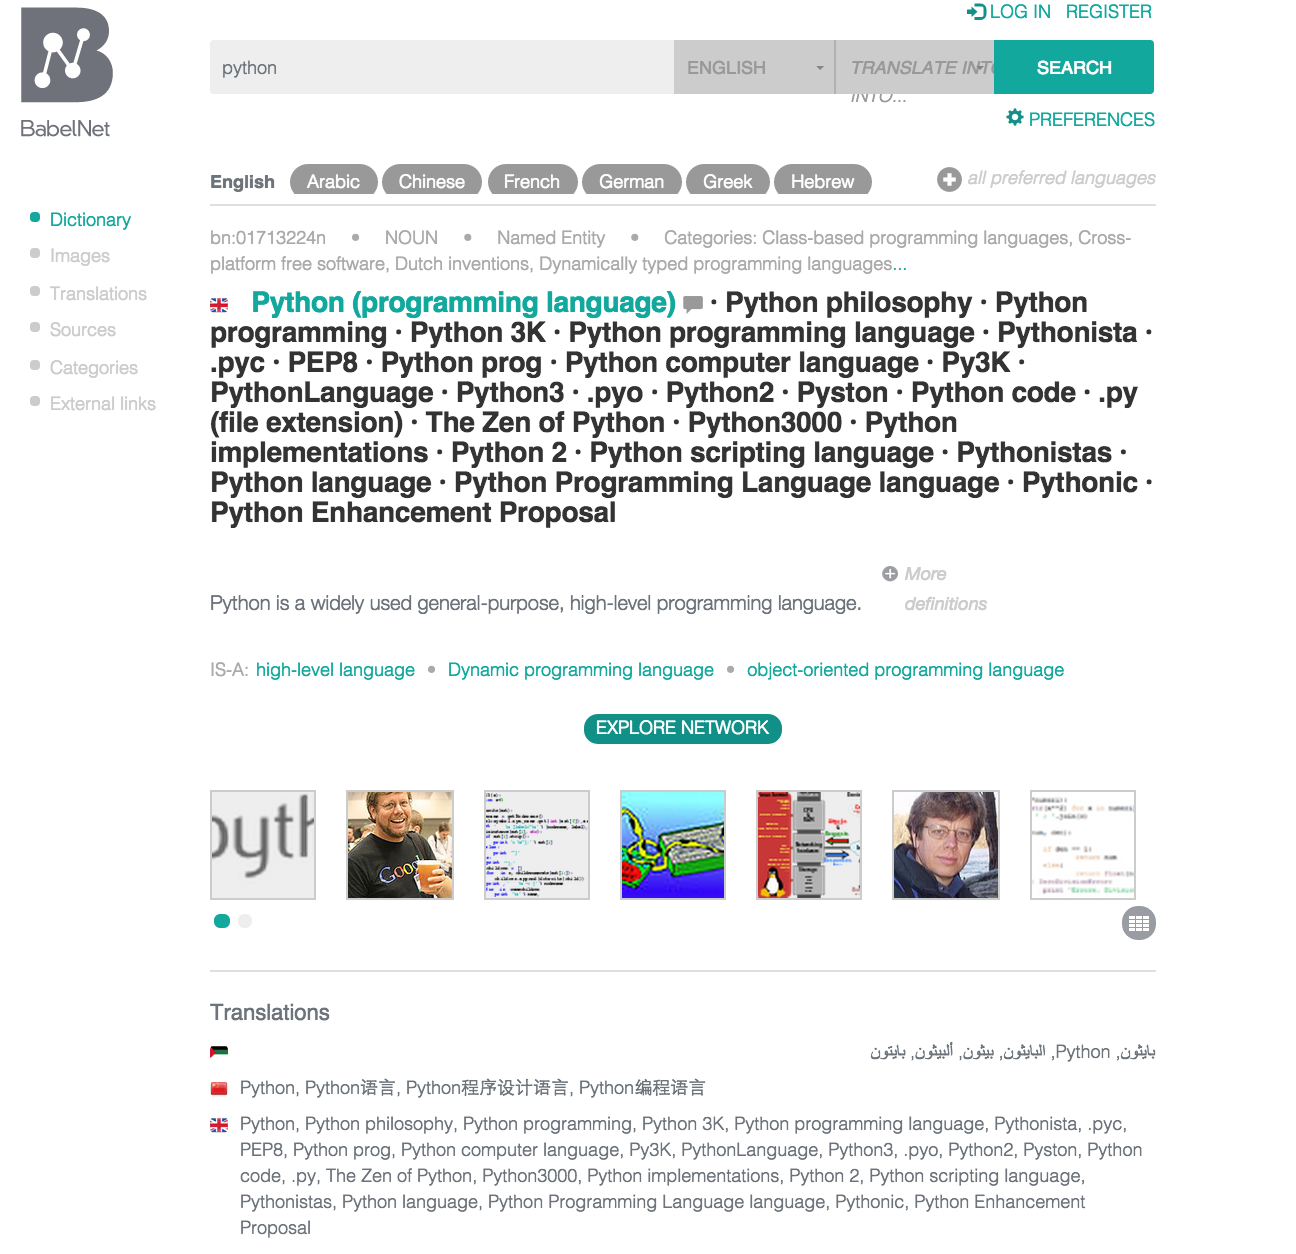
\includegraphics[height=0.7\textwidth]{./figures/babelnet2}
\end{figure}

\end{frame}





\begin{frame}
\frametitle{Semantic resources: ontology }

\begin{figure}
    \centering
        \includegraphics[width=1.0\textwidth]{../figures/ontology-new}
    \caption{ SUMO upper ontology: a part of the class hierarchy.}
    \label{fig:sumo}
\end{figure}
\end{frame}





\begin{frame}
\frametitle{Extraction of semantic resources from text }

\begin{figure}
\centering
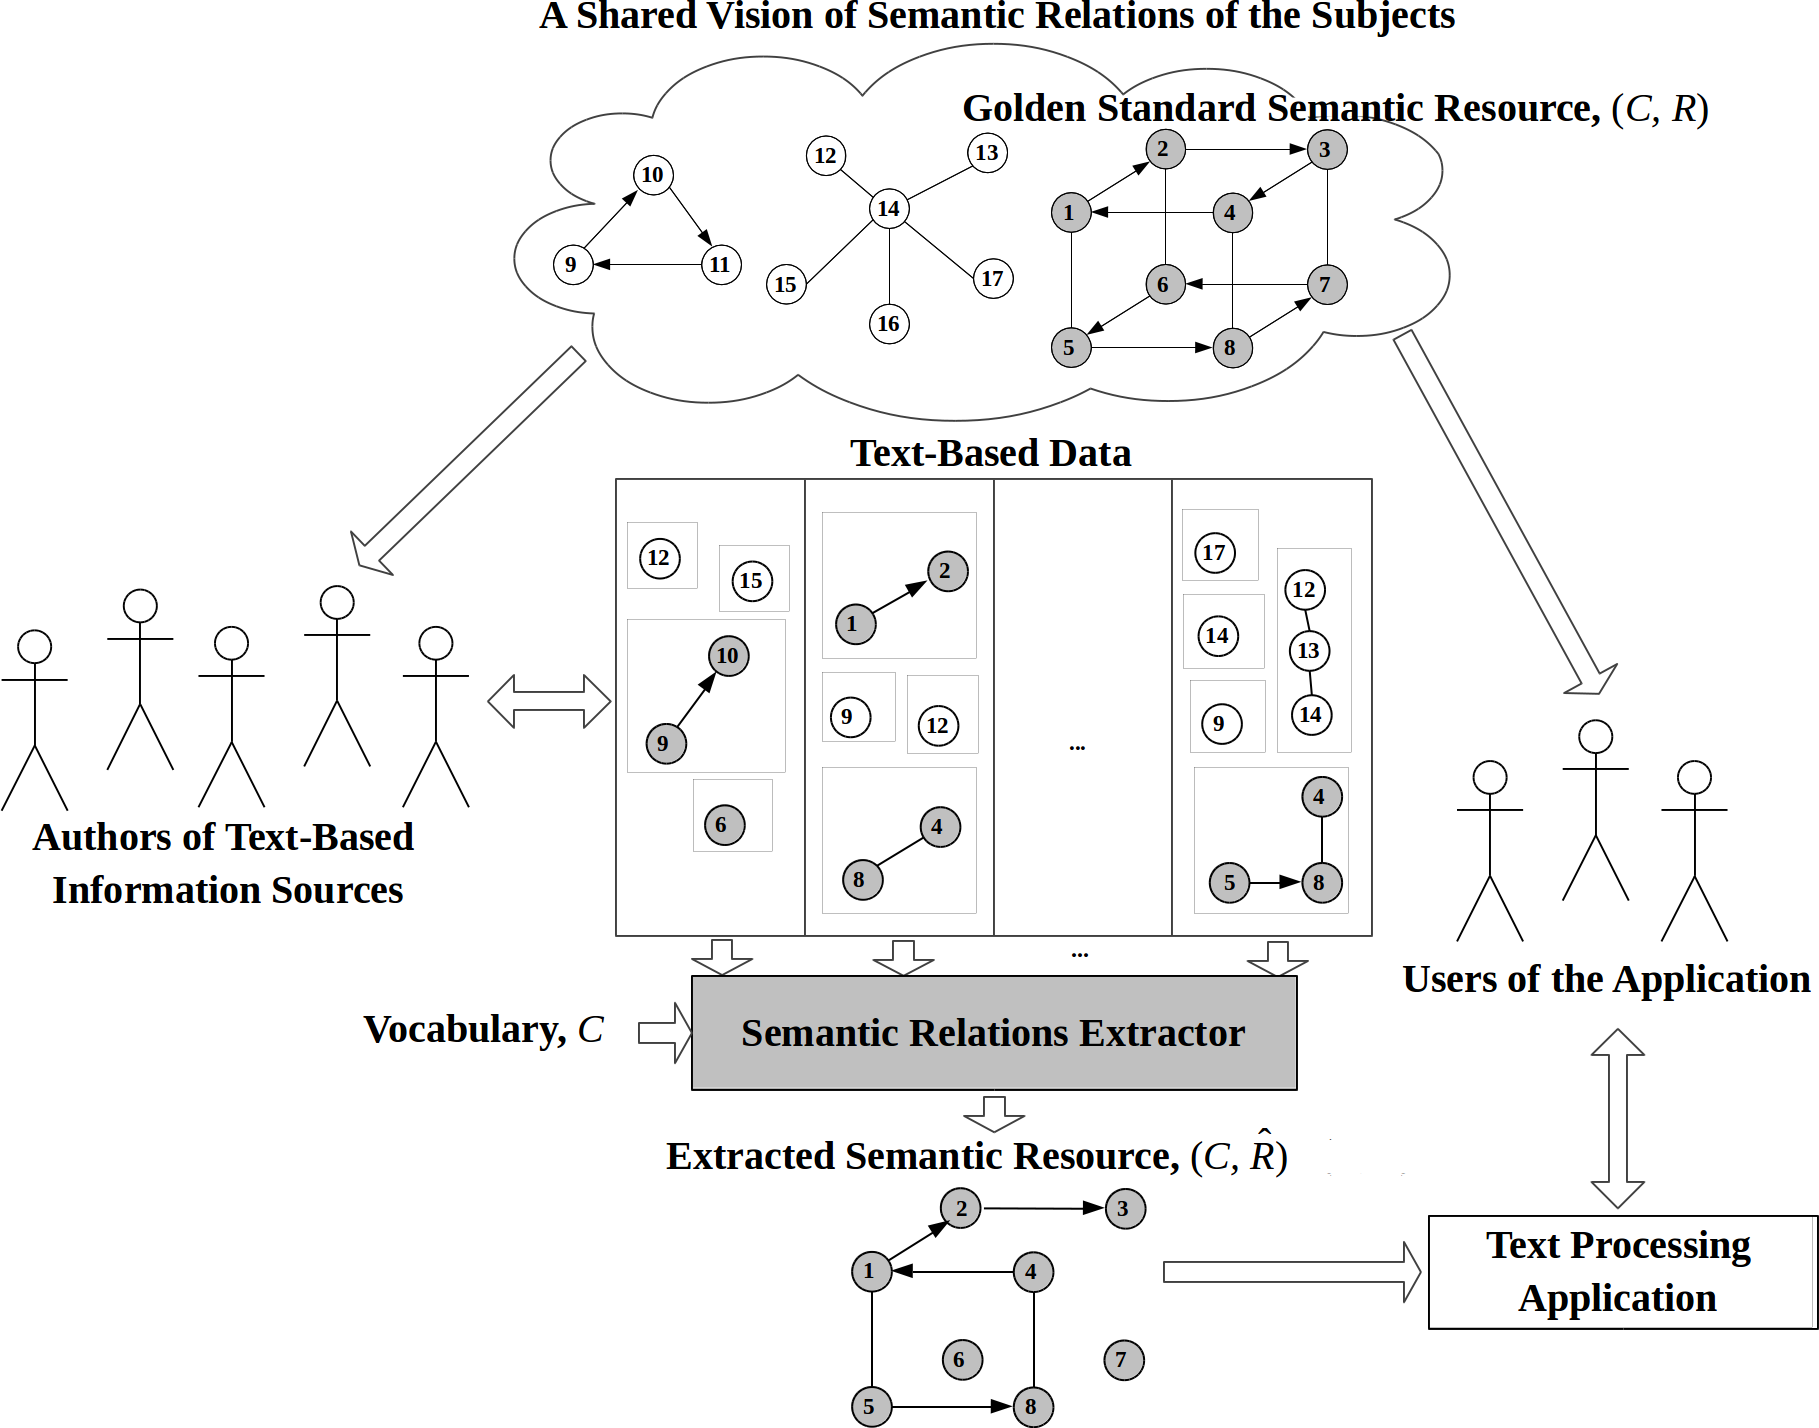
\includegraphics[width=0.8\textwidth]{../figures/extraction-3}

\label{fig:semantic-relations-extraction}
\end{figure}

\end{frame}








%%%%%%%%%%%%%%%%%%%%%%%%%%%%%%%%%%%%%%%%%%%%%%%%%
%%%%%%%%%%%%%%%%%%%%%%%%%%%%%%%%%%%%%%%%%%%%%%%%%
%%%%%%%%%%%%%%%%%%%%%%%%%%%%%%%%%%%%%%%%%%%%%%%%%

\section[Обзор метрик]{Обзор метрик семантической близости} 
\subsection{  }


\begin{frame}
\frametitle{Обзор метрик семантической близости}

\textbf{Публикации} 
\begin{itemize}
\item Panchenko A., \textbf{Similarity Measures for Semantic Relation Extraction.} PhD thesis. Universit\'{e} catholique de Louvain. 197
pages, 2013: \alert{Chapters 2.1, 3.1}. 
\item Panchenko A. \textbf{A Study of Heterogeneous Similarity Measures for Semantic Relation Extraction.} // In JEP-TALN-RECITAL 2012 — Grenoble (France), 2012.

\item ACL Anthology / Google Scholar: \alert{``semantic similarity measure''}, \alert{``semantic similarity''}. 
\end{itemize}
 
\end{frame}



\begin{frame}
\frametitle{Обзор метрик семантической близости}

\begin{figure}
\includegraphics[width=1.05\textwidth]{./../figures/measures-classification}
\end{figure}

\textbf{Публикации} (анализ 37 базовых метрик):
\begin{itemize}
\item Panchenko A., \textbf{Similarity Measures for Semantic Relation Extraction.} PhD thesis. Universit\'{e} catholique de Louvain. 197
pages, 2013, (Chapter 3). 
\item Panchenko A. \textbf{A Study of Heterogeneous Similarity Measures for Semantic Relation Extraction.} // In JEP-TALN-RECITAL 2012 — Grenoble (France), 2012. 
\end{itemize}
 
\end{frame}



%%%%%%%%%%%%%%%%%%%%%%%%%%%%%%%%%%%%%%%%%%%%%%%%%
\begin{frame}
\frametitle{Метрики, основанные на семантической сети}

 \textbf{Данные:} семантическая сеть WordNet 3.0, корпус SemCor.
    
 \textbf{Переменные:}
\begin{itemize}
\item $len(c_i,c_j)$ -- длина \textbf{кратчайшего пути} между $c_i$ и $c_j$
\item  $len(c_i, lcs(c_i,c_j))$ -- длина кратчайшего пути от $c_i$ до \textbf{ближайшего общего предка  (БОП)} слов $c_i$ и $c_j$

\item Ближайший Общий Предок (БОП) -- Lowest Common Subsumers (LCS) 

\item $len(c_{root}, lcs(c_i,c_j))$ -- длина кратчайшего пути от \textbf{корня} $c_{root}$ до БОП слов $c_i$ и $c_j$ (глубина БОП)
\item $P(c)$ --  \textbf{вероятность слова} $c$, оцененная из корпуса
\item  $P(lcs(c_i, c_j))$ -- \textbf{вероятность БОП} слов $c_i$ и $c_j$
\end{itemize}
    
    
\textbf{Метрики:} Инвертированная длина пути, Leacock-Chodorow, Wu-Palmer, 
 Resnik, Jiang-Conrath, Lin.
  
\end{frame}




\begin{frame}
\frametitle{Lowest common subsumer (LCS) }

\begin{figure}
\centering
\includegraphics[width=0.55\textwidth]{../figures/lcs-example}
\caption{Ближайшие общие предки в семантической сети.}
\end{figure}
    
\begin{itemize}
  \item $(car, food) \rightarrow object$
  \item $(beef, pork) \rightarrow meat$
  \item $(pork, coupe) \rightarrow object$
  \item $(vegetable, pork) \rightarrow food$
\end{itemize}

\end{frame}






\begin{frame}
\frametitle{Метрики, основанные на семантической сети}

\begin{itemize}

\item \textbf{Инвертированная длина пути}:

$$
s_{ij}=len(c_i,c_j)^{-1}.
$$

\item \textbf{LeacockChodorow}: 
$$
s_{ij}=-\log\frac{len(c_i,c_j)}{2h}.
$$

\item \textbf{Resnik}: 
$$
s_{ij}=-\log P(c_{ij}).
$$ 


\item \textbf{JiangConrath}: 
$$
d_{ij}= 2 \log P(c_{ij}) - (\log P(c_i) + \log P(c_j)).
$$

\end{itemize}

\end{frame}






\begin{frame}
\frametitle{Метрики, основанные на семантической сети}


\begin{itemize}

\item \textbf{Lin}: $$ s_{ij}= \frac{2 \log(P(c_{ij}))}{\log(P(c_i) + \log(P(c_j))  } $$

\item \textbf{WuPalmer}: 
$$ s_{ij}=\frac{2  len(c_{r},c_{ij})}{len(c_i,c_{ij})+len(c_j,c_{ij})+2\cdot len(c_{r},c_{ij})} $$
 
\end{itemize}
\end{frame}






\begin{frame}
\frametitle{Метрики, основанные на семантической сети}

\textbf{Инструменты}:

\begin{itemize}
\item WordNet::Similarity tool (Perl, command-line): \url{http://wn-similarity.sourceforge.net/}

\item NTLK (Python): \url{http://nltk.org}

\end{itemize}

\begin{figure}
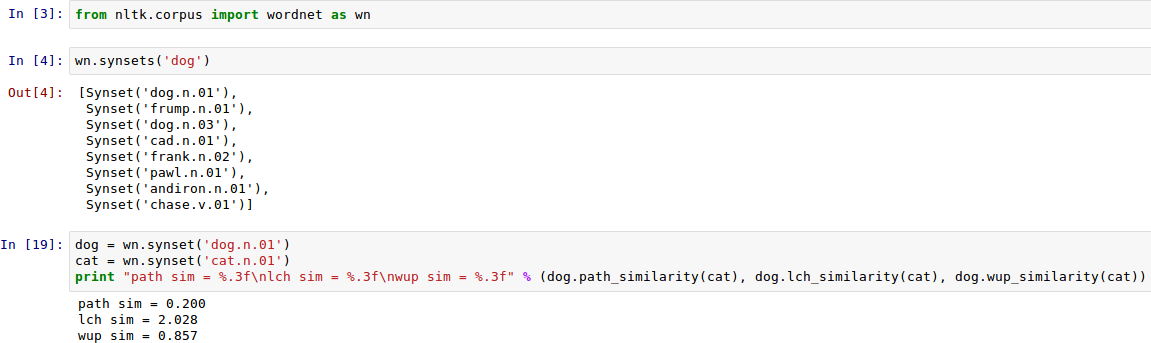
\includegraphics[width=1.0\textwidth]{./figures/python-example}
\end{figure}

\tiny{
Источник: \url{http://googlecode.com/svn-/trunk/doc/howto/wordnet.html}
}


\end{frame}







%%%%%%%%%%%%%%%%%%%%%%%%%%%%%%%%%%%%%%%%%%%%%%%%%
\begin{frame}
\frametitle{Метрики, основанные на Веб корпусе текстов }

\textbf{Данные:} количество документов возвращенных ИПС: Google, 
Yahoo, AltaVista, Bing, и т.п.
    
\textbf{Переменные:} 
\begin{itemize}
    \item $h_i$ -- \textbf{количество документов} возвращенных по запросу слова
    $"c_i"$
    \item $h_{ij}$ -- \textbf{количество документов} возвращенных по запросу $"c_i \text{ AND } c_j"$
\end{itemize}

\textbf{Метрики:} 
\begin{itemize}
\item Normalized Google Distance (NGD) (Cilibrasi and Vitanyi, 2007)
\item Pointwise Mutual Information - Information Retrieval (PMI-IR) (Turney,
2001)
\end{itemize}
\end{frame}








%%%%%%%%%%%%%%%%%%%%%%%%%%%%%%%%%%%%%%%%%%%%%%%%%
\begin{frame}
\frametitle{ Веб-метрики: пример }

 \begin{figure}
  \centering
   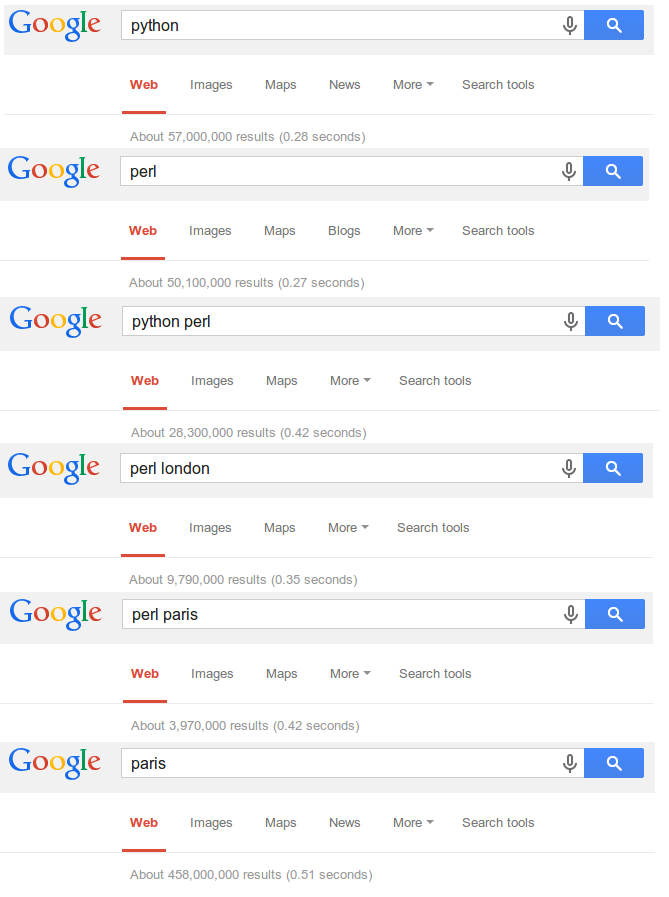
\includegraphics[width=0.5\textwidth]{./figures/google-web}
 \end{figure}

\end{frame}







\begin{frame}
\frametitle{Метрики, основанные на Веб корпусе текстов }

\begin{itemize}
\item \textbf{Normalized Google Distance (NGD)}: 
 
 $$ s_{ij}=\frac{max(log(h_i), log(h_j))-log(h_{ij})}{log(M)-min(log(h_i),log(h_j))} $$

\item \textbf{Pointwise Mutual Information Information Retrieval (PMIIR)}:
$$
s_{ij}= \log \frac{P(c_i,c_j)}{P(c_i) P(c_j)} = \log \frac{ \frac{h_{ij}}{\sum_{i,j} h_{ij}} }{ \frac{h_{i}}{\sum_{i,j} h_{ij}} \frac{h_{j}}{\sum_{i,j} h_{ij}} } \approx \log \frac{h_{ij} }{h_i h_j} .
$$

\end{itemize}

\end{frame}








%%%%%%%%%%%%%%%%%%%%%%%%%%%%%%%%%%%%%%%%%%%%%%%%%
\begin{frame}
\frametitle{Дистрибутивные метрики}

\textbf{Данные:} корпус, такой как Википедия или ukWaC

\begin{figure}
\centering
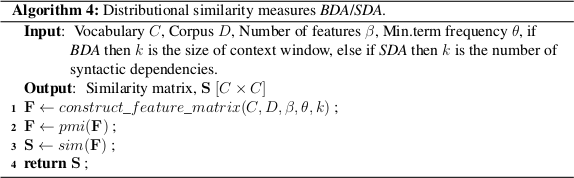
\includegraphics[width=0.8\textwidth]{./figures/dist-sem-algo}
\end{figure}

\textbf{Метрики:}
\begin{itemize}
    \item Bag-of-words Distributional Analysis (BDA) (Sahlgren, 2006)
    \item Syntactic Distributional Analysis (SDA) (Curran, 2003)
\end{itemize}
    
\end{frame} 
    
    
    
\begin{frame}
\frametitle{Дистрибутивные метрики}

\textbf{Переменные:} 
\begin{itemize}

\item $\textbf{f}_i$-- вектор признаков представляющий слово $c_i$, основанный на \textbf{контекстном окне}

\item $ \mathbf{f}^s_i$ -- вектор признаков представляющий слово $c_i$, основанный на \textbf{синтаксическом контекстном окне}
\begin{figure}
\includegraphics[width=0.9\textwidth]{./../figures/10-figure-3-gray}
\end{figure}

\begin{figure}
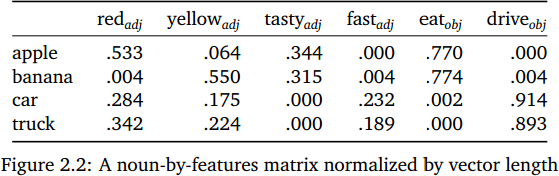
\includegraphics[width=0.6\textwidth]{./figures/sda-table}
\end{figure}

\tiny{\textbf{Источник}: Tim Van de Cruys, Mining for Meaning, PhD thesis (2010)}

   
\end{itemize}
    
    
\end{frame}
    




\begin{frame}
\frametitle{Другие метрики, основанные на корпусе текстов}

\textbf{Данные:} корпус, такой как Википедия или ukWaC
    
    
\textbf{Метрики:}
\begin{itemize} 
\item Латентно-cемантический анализ (LSA) (Landauer and Dumais, 1997)
\item Вероятностные модели (pLSA, LDA и др.) (Griffiths et al., 2007)
\item NGD и PMI-IR (Veksler et al., 2008)
\item \ldots
\end{itemize}
    
\end{frame}



\begin{frame}
\frametitle{Латентно-семантический анализ}
\textbf{Latent Semantic Analysis (LSA)} (Landauer and Dumais, 1997):

\begin{enumerate}
\item Representing the corpus $D$ as an $N \times M$ term-document matrix $\mathbf{F}$.

% An element $f_{ij} \in \mathbf{F}$ of this matrix contains frequency of the word $w_i$ in the document $d_j \in D$. 

\item  Normalization of the matrix $\mathbf{F}$ with TF-IDF:
$$
f_{ij}^\prime = \frac{f_{ij}}{\sum_i f_{ij}} \cdot log \frac{|D|}{|d \in D : w_i \in d|},
$$


\item Singular value decomposition of $\mathbf{D}$: $ \mathbf{D} = \mathbf{U} \Sigma \mathbf{V}^T.$

\item Low-rank approximation of the matrix $\mathbf{U}$ with a reduced $M \times k$ matrix $\mathbf{U}_k$ by retaining only the first $k$ column of the $\mathbf{U}$. 

\item Calculation of similarities between terms $c_i$ and $c_j$ as a cosine between respective columns of $\mathbf{U}_k$ ($\mathbf{u}^k_i$ and $\mathbf{u}^k_i$):

$$
s_{ij} = \frac{\mathbf{u}^k_i \cdot \mathbf{u}^k_j}{||\mathbf{u}^k_i|| ||\mathbf{u}^k_j ||}.
$$

\end{enumerate}

\end{frame}







\begin{frame}
\frametitle{Латентно-семантический анализ}

\begin{itemize}

\item $\mathbf{U}$ is an $M \times M$ matrix which columns are the orthogonal eigenvectors of $\mathbf{D D}^T$
\item  $\mathbf{V}^T$ is an $N \times N$ matrix which columns are the orthogonal eigenvectors of $\mathbf{D}^T \mathbf{D}$

\item $\Sigma$ is an $M \times N$ diagonal matrix:

$$
\Sigma = \begin{pmatrix}
  \sigma_{11} & \ldots & 0 \\
  \vdots  & \ddots & \vdots  \\
  0 & \cdots & \sigma_{nn}
 \end{pmatrix}.
$$

\item The $i$-th element on the diagonal $\sigma_{ii} = \sqrt{\lambda_i}$, where $\lambda_i$ is an eigenvalue of $\mathbf{D D}^T$. 

\item The eigenvalues are ordered, such that $\lambda_i \geq \lambda_{i+1}$.  

\end{itemize}

\tiny{\textbf{Источник}: Manning et al. Introduction to information retrieval (2008), p.374.}

\end{frame}




\begin{frame}
\frametitle{Латентно-семантический анализ}

\begin{figure}
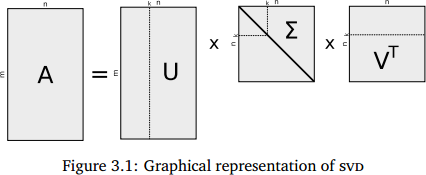
\includegraphics[width=0.8\textwidth]{./figures/lsa}
\end{figure}

\tiny{\textbf{Источник}: Tim Van de Cruys, Mining for Meaning, PhD thesis (2010)}

\end{frame}




%%%%%%%%%%%%%%%%%%%%%%%%%%%%%%%%%%%%%%%%%%%%%%%%%
\begin{frame}
\frametitle{Метрики, основанные на определениях}

\textbf{Данные:} определения из WordNet, Википедии, Викисловаря или любого
другого словаря.
    
\textbf{Переменные:}
\begin{itemize}
        \item $gloss(c_i)$ -- \textbf{определение} слова $c_i$;
        \item $\mathbf{f}_i$ \textbf{вектор признаков}, построенный из $gloss(c_i)$;
        \item $\mathbf{f}_i$ -- \textbf{вектор признаков} $c_i$, вычисленный на
        корпусе из всех определений методом контекстного окна;
        
        \item $exist(c_i, c_j)$ -- наличие связи между $c_i$ и $c_j$ в словаре.
\end{itemize}

\textbf{Метрики:}
\begin{itemize}
  \item ExtendedLesk (Banerjee and Pedersen, 2003)
  \item GlossVectors (Patwardhan and Pedersen, 2006)
  \item DefVectors (Panchenko et al., 2012)
  
\end{itemize}

\end{frame}





\begin{frame}
\frametitle{Метрики, основанные на определениях: Extended Lesk}

\begin{itemize}
\item relies on the gloss similarity of terms $c_i$ and $c_j$
\item relies on gloss similarity of all terms related to $c_i$ and $c_j$  

$$
s_{ij}=\sum_{c_i \in C_i}\sum_{c_j \in C_j} sim_g(c_i,c_j),
$$
\item $sim_g$ is a gloss-based similarity measure and set $C_i$ includes concept $c_i$ and all concepts directly related to it. 
\end{itemize}

\end{frame}


\begin{frame}
\frametitle{Метрики, основанные на определениях: GlossVectors}


\begin{itemize}
\item a cosine between vectors $\mathbf{v}_i$ and $\mathbf{v}_j$ representing concepts $c_i$ and $c_j$

\item a vector $\mathbf{v}_i$ is a sum of context vectors representing all words from the definition of $c_i$ and the definitions of terms related to $c_i$:

$$
s_{ij} =  \frac{\mathbf{v}_i \cdot \mathbf{v}_j}{||\mathbf{v}_i|| ||\mathbf{v}_j||} \text{ where } \mathbf{v}_i = \sum_{ \forall j : c_j \in G_i  } \mathbf{f}_j.
$$

\item $\mathbf{f}_j$ is a context vector, derived from the corpus of all glosses 
\item $G_i$ is concatenation of glosses of the concept $c_i$ and all concepts which are directly related to it.

\end{itemize}

\end{frame}





\begin{frame}
\frametitle{Сравнение базовых метрик семантической близости}



\begin{figure}
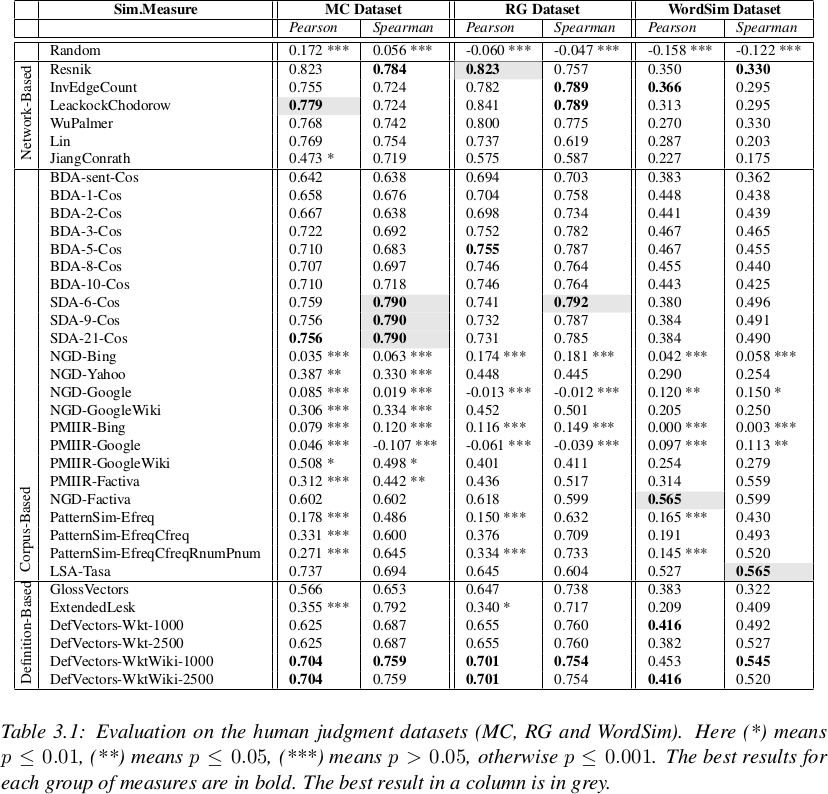
\includegraphics[width=0.69\textwidth]{./figures/overview-table1}
\end{figure}
   
\end{frame}





\begin{frame}
\frametitle{Сравнение базовых метрик семантической близости}

\begin{figure}
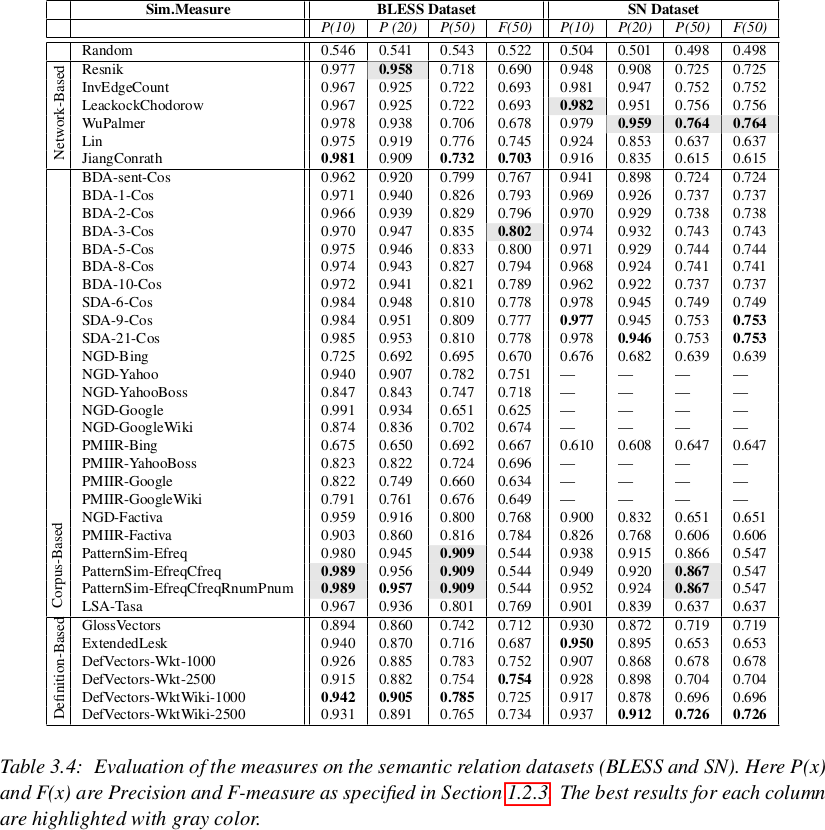
\includegraphics[width=0.65\textwidth]{./figures/overview-table2}
\end{figure}
   
\end{frame}






\begin{frame}
\frametitle{Сравнение: лучшие базовые метрики}

\begin{figure}
\includegraphics[width=1.05\textwidth]{./../figures/best}

\end{figure}

\begin{itemize}
  \item Каждая метрика излекает много \alert{ко-гипонимов}: 
  \begin{itemize}
  \item $\langle Canon, Nikon \rangle$,
  \item $\langle Lamborghini, Ferrari \rangle$,
  \item $\langle Obama, Romney \rangle$.
\end{itemize}
\end{itemize}
   
\end{frame}





\begin{frame}
\frametitle{Резюме}

\begin{block}{Основные ресурсы для построения метрик:}
\begin{itemize}
  \item семантические сети и тезаурусы;
  \item корпуса текстов;
  \item Веб корпус текстов;
  \item определения из словарей и энциклопедий. 
\end{itemize}
\end{block}   


\begin{block}{Метрики \textbf{дополняют друг друга} в терминах:}
\begin{itemize}
  \item лексического покрытия;
  \item точности;
  \item типов извлекаемых отношений. 
\end{itemize}
\end{block}   

\end{frame}





\begin{frame}
\frametitle{Программное обеспечение}

\begin{itemize}
  \item \textbf{Semantic Vectors:} \url{https://code.google.com/p/semanticvectors/}
  \item \textbf{S-Space Package:} \url{https://code.google.com/p/airhead-research/}
  \item \textbf{WordNet::Similarity:} \url{http://wn-similarity.sourceforge.net}
  \item \textbf{NLTK:} \url{http://nltk.googlecode.com/svn/trunk/doc/howto/wordnet.html}
  \item \textbf{WikiRelate!}
  \item \textbf{PatternSim / Serelex:} \url{http://serelex.cental.be}
  \item \textbf{Метрики, основанные на Веб корпусе:} \url{http://cwl-projects.cogsci.rpi.edu/msr}
  \item \textbf{LSA:} \url{http://lsa.colorado.edu}
  \item \textbf{DefVectors:} \url{http://github.com/jgc128/defvectors}
\end{itemize}

\end{frame}

   
\section[PatternSim]{Метрика основанная на лексико-синтаксических шаблонах}

\subsection{}

\begin{frame}
\frametitle{Публикации}

\begin{itemize}
  \item Hearst, M. A. Automatic acquisition of hyponyms from large text corpora. In ACL,
pages 539–545, 1992. 
\item Panchenko A., Morozova O., Naets H. \textbf{A Semantic Similarity Measure Based on Lexico-Syntactic Patterns.} In Proceedings of KONVENS 2012, pp.174--178, 2012
\item Panchenko A., Romanov P., Morozova O., Naets H., Philippovich A., Fairon
C. \textbf{Serelex: Search and Visualization of Semantically Related Words}.
In Proceedings of the 35th European Conference on Information Retrieval (ECIR 2013).

\item Панченко А., Романов П., Романов А.,  Филиппович А.,
Филиппович Ю., Морозова О. \textbf{Серелекс: поиск и визуализация
семантически связанных слов}. Анализ Изображений, Сетей и Текстов (АИСТ), Интуит, 2013
\end{itemize}
\end{frame}

\begin{frame}
\frametitle{Демо}

\begin{itemize}
  \item {\bf \url{http://serelex.cental.be/} }
  
\begin{figure}  
    \centering
        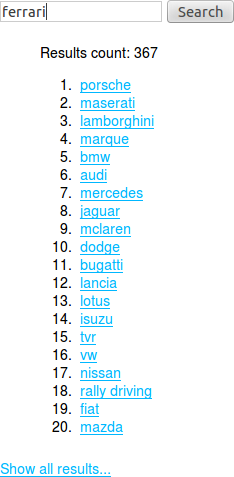
\includegraphics[height=0.6\textwidth]{figures/serelex}
        
\includegraphics[height=0.5\textwidth]{figures/spacer}
        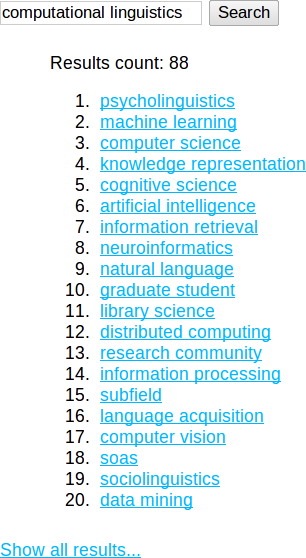
\includegraphics[height=0.6\textwidth]{figures/serelex-2}
        \end{figure}
\end{itemize}
\end{frame}


\begin{frame}
\frametitle{Лексико-синтаксические паттерны}

\begin{itemize}
  \item 18 паттернов извлекающих \textbf{гиперонимы},
  \textbf{ко-гипонимы} и \textbf{синонимы}
\begin{figure}  
    \centering
        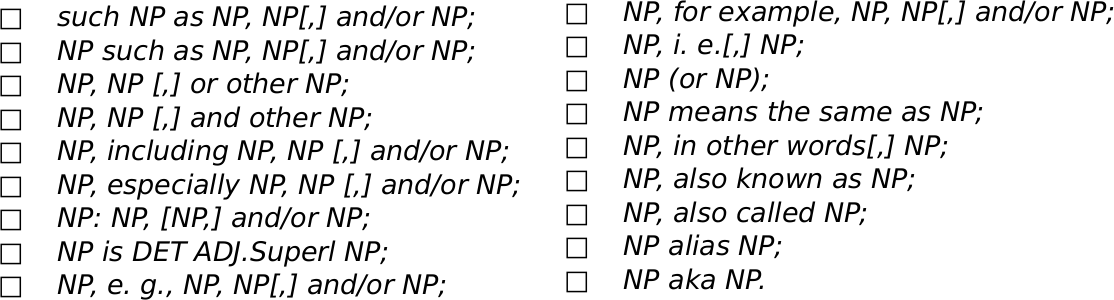
\includegraphics[width=1.0\textwidth]{figures/patterns}
    \end{figure}
\end{itemize}

\end{frame}

\begin{frame}
\frametitle{Основной каскад преобразователей}

\begin{itemize}
  \item Каскад конечных автоматов (FST)
  \item В формате \texttt{Unitex}: \url{http://igm.univ-mlv.fr/~unitex/}
  
\begin{figure}  
    \centering
        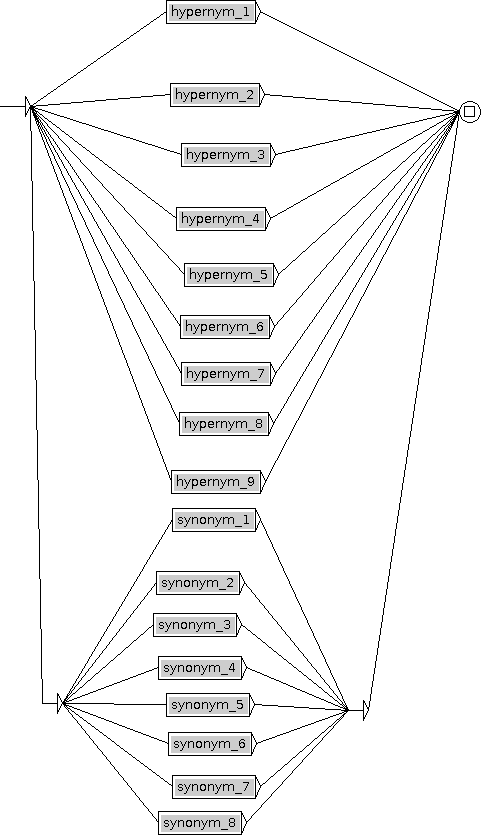
\includegraphics[width=0.3\textwidth]{figures/main-graph}
    \end{figure}
\end{itemize}

\end{frame}

\begin{frame}
\frametitle{Пример реализации паттерна в виде автомата}

\begin{figure}  
    \centering
        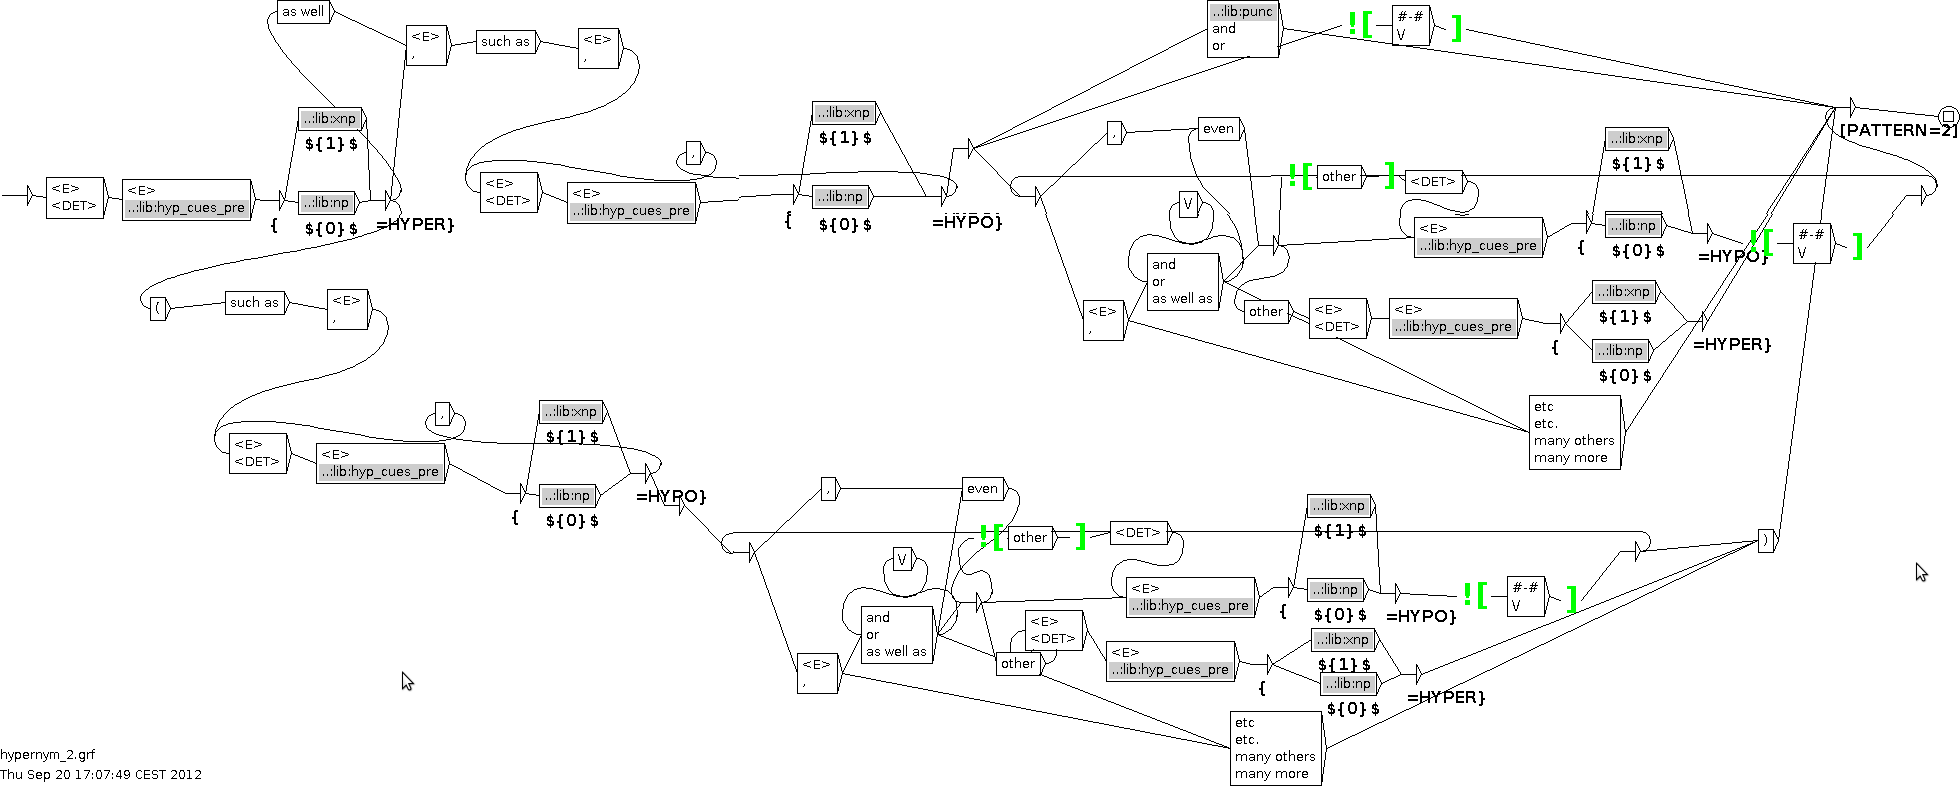
\includegraphics[width=1.0\textwidth]{figures/pattern2}
    \end{figure}

\begin{itemize}
  \item Паттерны, основанные на автоматах позволяют учесть лингвистическую вариацию, сохранив
  точность
      \item В отличие от паттернов основанных на строках (Bollegala et al., 2007)
    
\end{itemize}

\end{frame}






\begin{frame}
\frametitle{PatternSim: основные этапы}


\textbf{Паттерны извлекают конкордансы}

\begin{itemize}
  \item \texttt{such diverse \{[occupations]\} as
  \{[doctors]\}, \{[engineers]\} and \{[scientists]\}[PATTERN=1]}
  \item \texttt{such \{non-alcoholic [sodas]\} as \{[root beer]\} and \{[cream soda]\}[PATTERN=1]}
  \item \texttt{\{traditional[food]\}, such as \{[sandwich]\},\{[burger]\}, and \{[fry]\}[PATTERN=2]}
\end{itemize}

\end{frame}






\begin{frame}
\frametitle{PatternSim: основные этапы}

\textbf{Корпус} Wikipedia+ukWaC: $2.9\cdot10^{12}$ токенов

\begin{figure}  
\centering
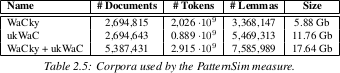
\includegraphics[width=0.7\textwidth]{figures/patternsim-table}
\end{figure}


\textbf{Количество извлечений}

\begin{itemize}
  \item Wikipedia -- 1.196.468 
  \item ukWaC -- 2.227.025 
  \item WaCypedia+ukWaC -- 3.423.493
\end{itemize}

\end{frame}





\begin{frame}
\frametitle{Метрика семантической близости PatternSim }

\begin{figure}  
\centering
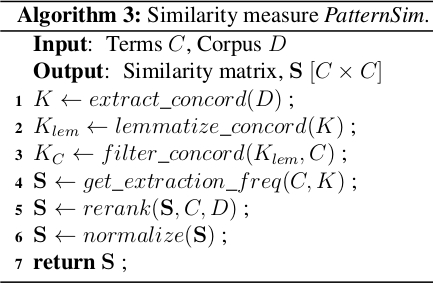
\includegraphics[width=0.6\textwidth]{figures/patternsim-algo}
\end{figure}

\end{frame}



\begin{frame}
\frametitle{Вычисление подобия: rerank}


\begin{itemize}
  \item \textbf{Efreq}: мера подобия равна количеству извлеченных отношений
  $$ s_{ij} = s_{ij} $$
  
  \item \textbf{Efreq-Cfreq}: нормализация по частоте слов
  
  $$ s_{ij} = \frac{P(c_i,c_j)}{P(c_i)P(c_j)} $$ 
    
    \begin{itemize}
    \item $P(c_i,c_j)=\frac{e_{ij}}{\sum_{ij}e_{ij}}$ -- вероятность извлечения
отношения $\langle c_i,c_j \rangle$, где $e_{ij}$ -- частота
взаимной встречаемости слов $c_i$ и $c_j$ во множестве конкордансов

\item $P(c_i)= \frac{f_i}{\sum_i f_i}$ -- вероятность слова $c_i$, где $f_i$
-- частота $c_i$

\end{itemize}
    
\end{itemize}

\end{frame}


\begin{frame}
\frametitle{Вычисление подобия: }
  
\begin{itemize}
  
\item \textbf{Efreq-Rnum-Cfreq-Pnum}:
  
$$s_{ij} = \sqrt{p_{ij}} \cdot \frac{2\cdot\mu_b }{b_{i*}+b_{*j}} \cdot \frac{P(c_i,c_j)}{P(c_i)P(c_j)}.$$

\begin{itemize}

\item $P(c_i,c_j)=\frac{e_{ij}}{\sum_{ij}e_{ij}}$ -- вероятность извлечения
отношения $\langle c_i,c_j \rangle$, где $e_{ij}$ -- частота
взаимной встречаемости слов $c_i$ и $c_j$ во множестве конкордансов

\item $P(c_i)= \frac{f_i}{\sum_i f_i}$ -- вероятность слова $c_i$, где $f_i$
-- частота $c_i$
\item $b_{i*} = \sum_{j:e_{ij} \geq \beta} 1$ -- количество извлечений слова
$c_i$ с частотой $\geq \beta$,  где $\mu_b = \frac{1}{|C|}\sum_{i=1}^{|C|}
b_{i*}$ -- среднее количество извлечений для отдельного слова

\item $p_{ij} \in [1;18]$ -- количество отдельных паттернов которые извлекли
отношение $\langle c_i, c_j \rangle$
 
\end{itemize}
\end{itemize}

\end{frame}






\begin{frame}
\frametitle{Ранжирование семантических отношений}

\begin{itemize}
  \item Точность \textbf{сравнима или лучше} чем у аналогов;
  \item Полнота \textbf{меньше} чем у аналогов.
\end{itemize}

\begin{figure}  
    \centering
    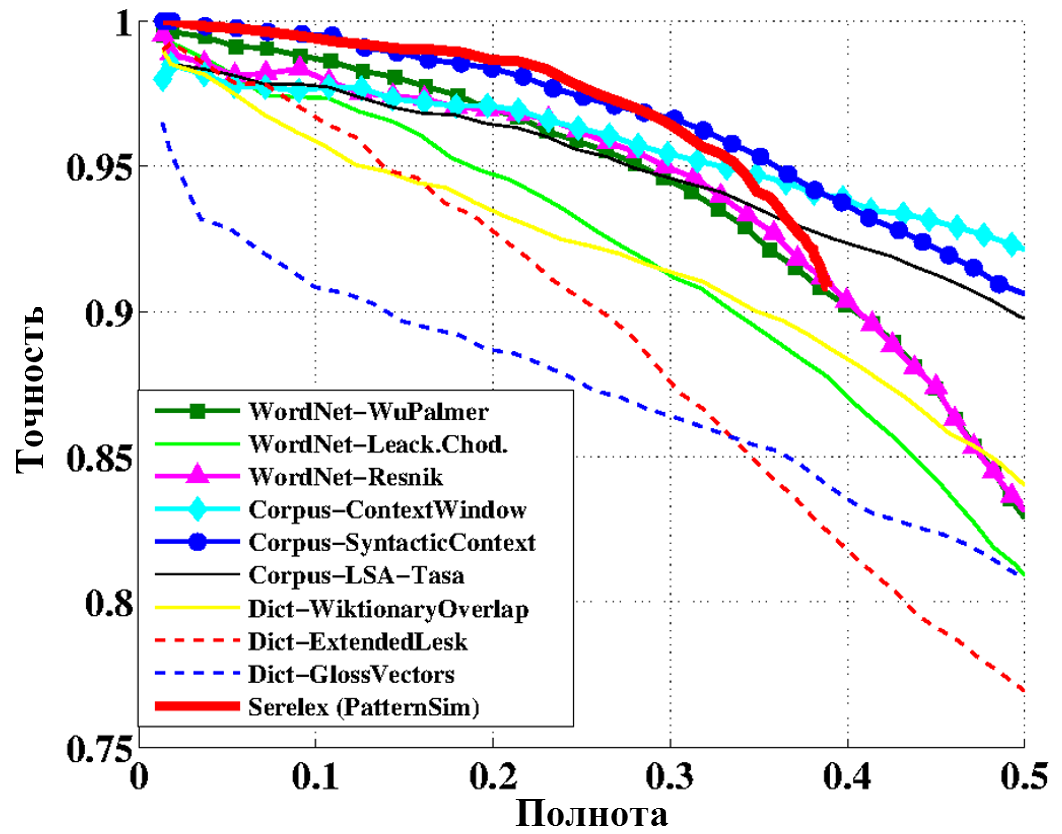
\includegraphics[width=0.6\textwidth]{pr}
    \caption{График точность-полнота (коллекция BLESS).
    }
\end{figure}

\end{frame}








\begin{frame}
\frametitle{Извлечение семантических отношений}
  \begin{columns}[T]
    \begin{column}{.4\textwidth}
     
% Your text here
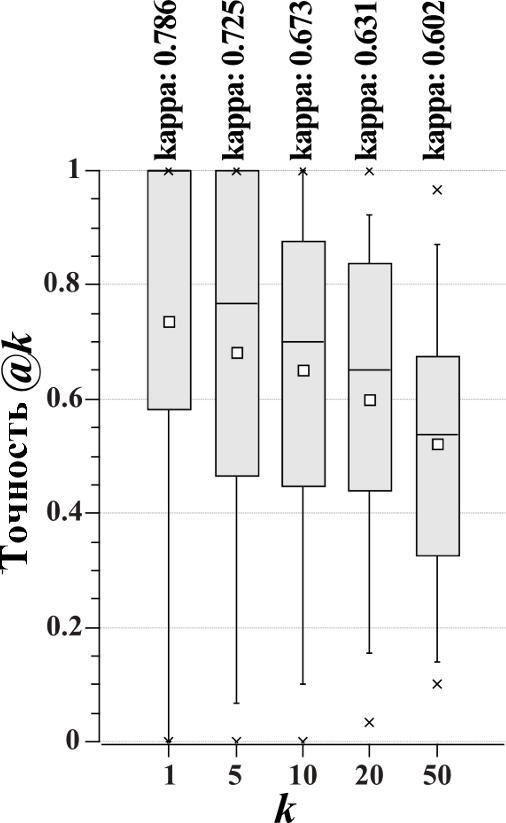
\includegraphics[width=0.85\textwidth]{./kappa}
    
    \end{column}
    \begin{column}{.6\textwidth}
    %\begin{block}{Your image}
\begin{itemize}
  %\item 49 words, three binary annotations;
  \item Точность@1 $\approx 0.80$;
  \item ``Хорошее'' лексическое покрытие:
  
\end{itemize}

\begin{figure}
\includegraphics[width=0.95\textwidth]{./../figures/wordnet-vs-serelex}
\end{figure}
      
    \end{column}
  \end{columns}
\end{frame}






\begin{frame}
\frametitle{Сравнение результатов базовых метрик и PatternSim}

\begin{figure}  
\centering
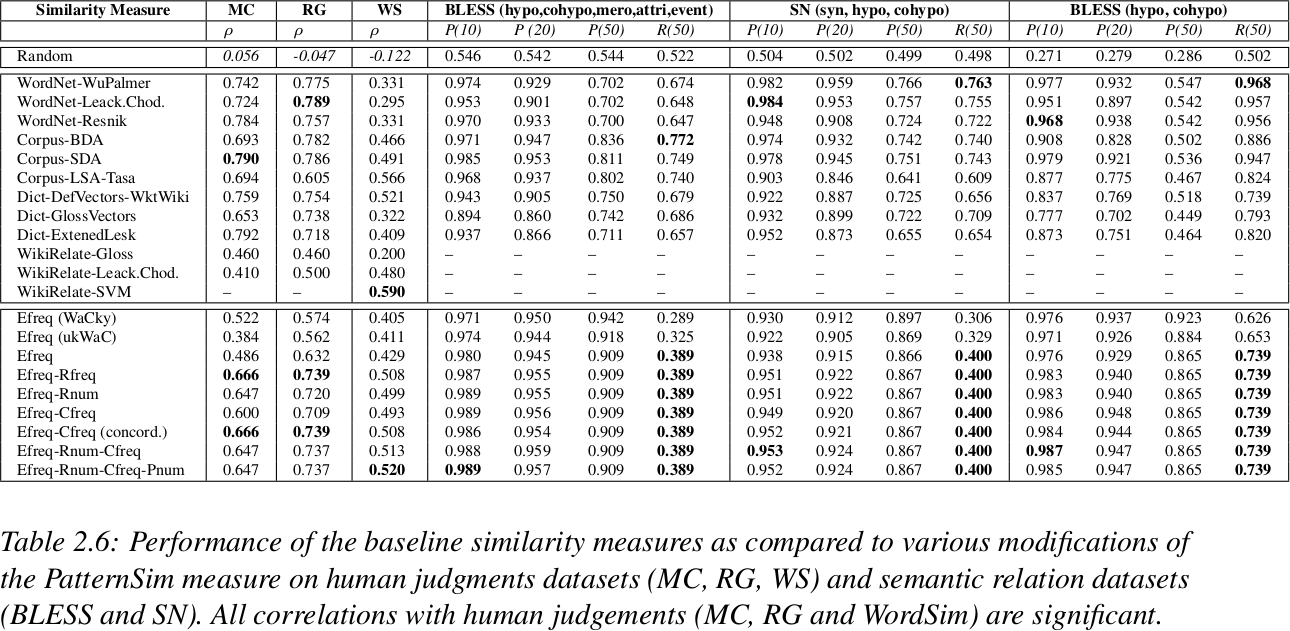
\includegraphics[width=0.9\textwidth]{figures/patternsim-results-table}
\end{figure}

\end{frame}




\section[HybridSim]{Гибридная метрика семантической близости}

\subsection{}

\begin{frame}
\frametitle{Публикациии}
\begin{itemize}
\item Panchenko A., Morozova O. \textbf{A Study of Hybrid Similarity Measures
for Semantic Relation Extraction.} // Innovative Hybrid Approaches to the Processing of Textual Data Workshop, EACL 2012 — Avignon (France), 2012 — pp. 10–18 
\item Panchenko A., \textbf{Similarity Measures for Semantic Relation
Extraction.} PhD thesis. Universit\'{e} catholique de Louvain. 197
pages, 2013, (Chapter 4). 

\item Panchenko A. \textbf{A Study of Heterogeneous Similarity Measures for
Semantic Relation Extraction.} // In JEP-TALN-RECITAL 2012 — Grenoble (France), 2012 — pp. 29–42.
\end{itemize}
\end{frame}


%### A multitude of \textbf{complimentary measures} were proposed to extract synonyms, hypernyms,
%and co-hyponyms

%### Most of them are based on \textbf{one} of the \textbf{5 key approaches}: 
%\begin{enumerate}
%\item distributional analysis (Lin, 1998b)
%\item web as a corpus (Cilibrasi and Vitanyi, 2007)
%\item lexico-syntactic patterns (Bollegala et al., 2007)
%\item semantic networks (Resnik, 1995)
%\item definitions of dictionaries or encyclopedias (Zesch et al., 2008a)
%\end{enumerate}

%\item Some attempts were made to \textbf{combine measures} (Curran, 2002; Cederberg and Widdows, 2003; Mihalcea et al., 2006;
%Agirre et al., 2009; Yang and Callan, 2009)

%### \item However, most studies are still \textbf{not taking into account} all 5 existing extraction approaches.


\begin{frame}
\frametitle{Отдельные и гибридные метрики}

\begin{figure}
\centering
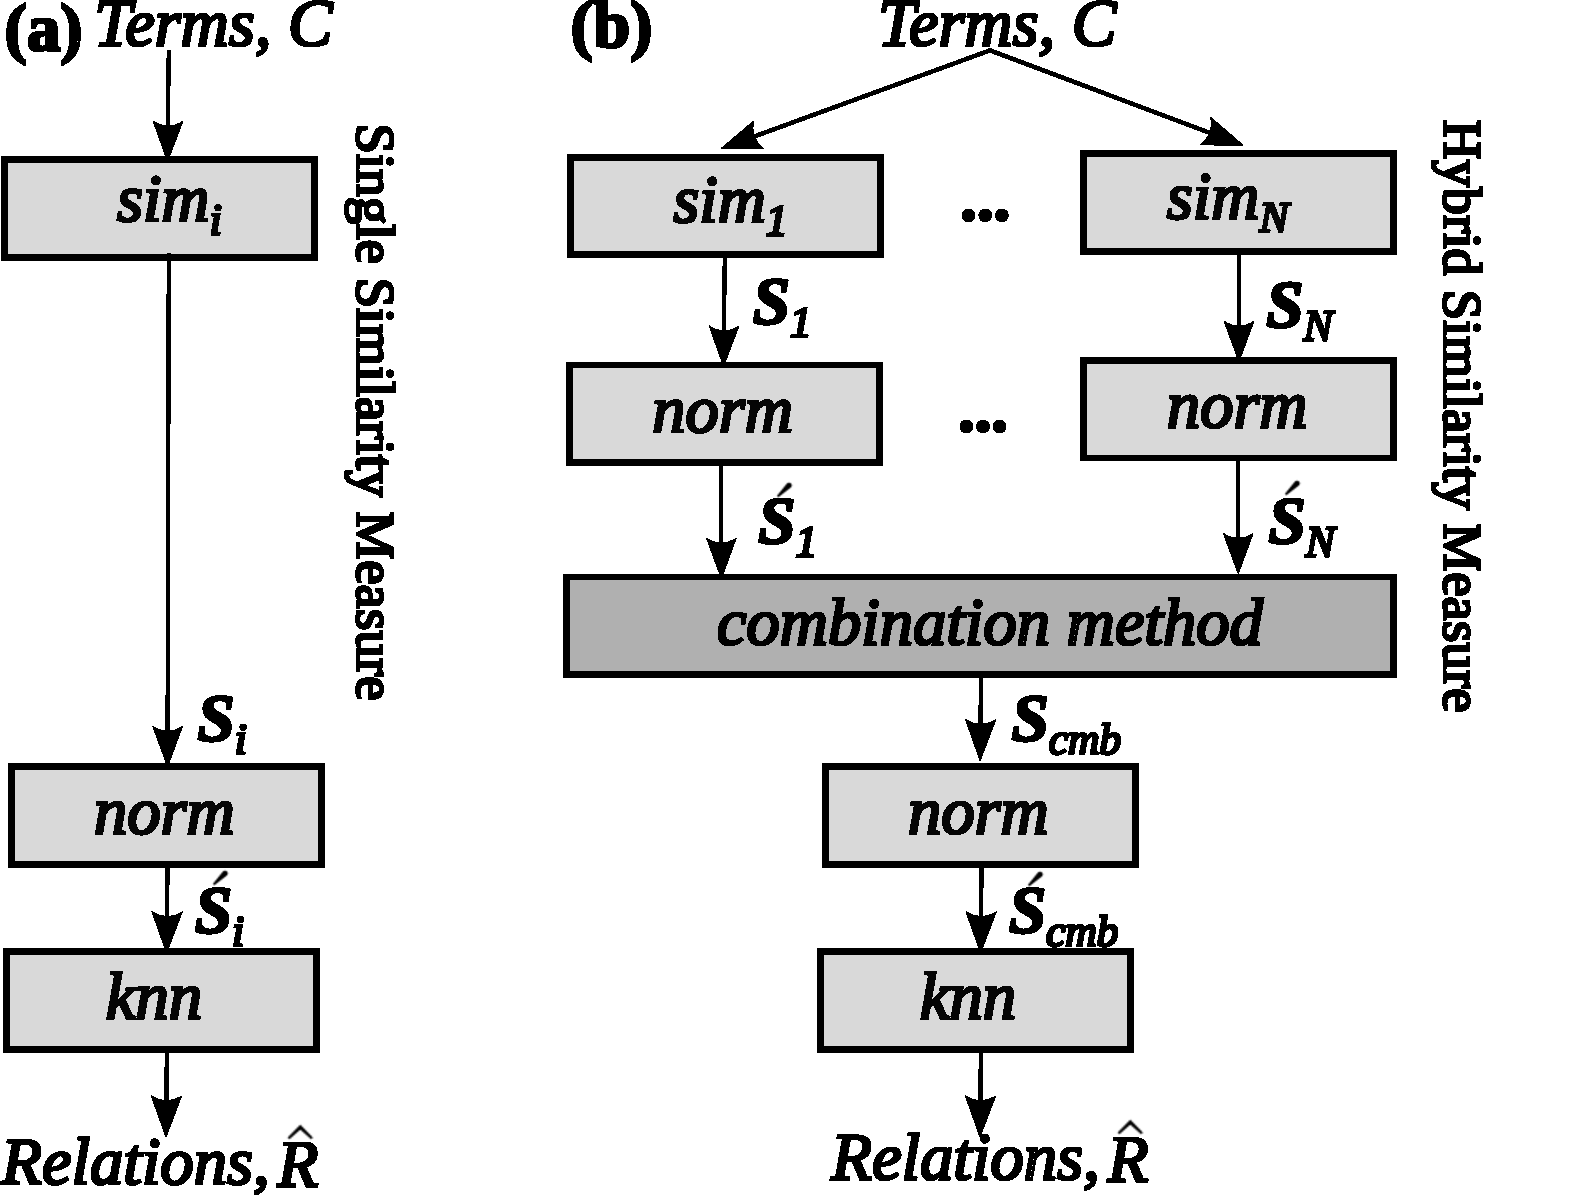
\includegraphics[width=0.65\textwidth]{./../figures/papers/4/src/figures/single-and-hybrid-2}
\caption{Система извлечения семантических отношений основанная на:
\begin{itemize}
\item \textbf{(a)} \textbf{отдельной} метрике;
\item \textbf{(b)} \textbf{гибридной} метрике. 
\end{itemize}}
\end{figure}
\end{frame}





\begin{frame}
\frametitle{16 признаков = 16 отдельных метрик}

    \begin{itemize}
    
    \item 5 метрик основанных на \textbf{семантических сетях}:
    \begin{enumerate}
      \item WuPalmer;
      \item Leacock and Chodorow;
      \item Resnik;
      \item Jiang and Conrath;
      \item Lin.
    \end{enumerate} 
    \item 3 метрики, основанные на \textbf{Веб корпусе} (NGD-Yahoo/Bing/Google);
        
    \item 5 метрики, основанные на \textbf{корпусе текстов}: 
    \begin{itemize}
      \item 2 дистрибутивных (BDA, SDA)
      \item 1 лексико-синтаксические шаблоны (PatternSim)
      \item 2 другие (LSA, NGD-Factiva)
    \end{itemize}
    
    \item 3 метрики, основанные на \textbf{определениях} 
    \begin{enumerate}
      \item ExtendedLesk;
      \item GlossVectors;
      \item DefVectors-WktWiki.
    \end{enumerate}
     
\end{itemize}

\end{frame}







\begin{frame}
\frametitle{Методы комбинирования без учителя}

\item $s_{ij}^k \in [0;1]$ -- попарное семантическое подобие слов $w_i$ и $w_j$, вычисленное с помощью $k$-й метрики $\mathbf{S}_k$.
 
\begin{block}{Mean}

Среднее между $K$ попарными подобиями слов:

$$s_{ij}^{cmb}= \frac{1}{K}\sum_{k=1,K} s_{ij}^k;$$

\end{block} 

\begin{block}{Mean-Nnz} 
Среднее между $K$ попарными подобиями слов больше нуля:

$$s_{ij}^{cmb}= \frac{1}{|k:s_{ij}^k >0,k=1,K|}\sum_{k=1,K} s_{ij}^k;$$

\end{block} 
\end{frame}







\begin{frame}
\frametitle{Методы комбинирования без учителя}


\begin{block}{Mean-Zscore}
Среднее между нормированными попарными подобиями слов (Z-score):

$$\mathbf{S}_{cmb} = \frac{1}{K} \sum_{k=1}^K \frac{\mathbf{S}_k -\mu_k}{\sigma_k};$$

где $\mu_k$ и $\sigma_k$ среднее и стандартное отклонение значений $k$-й метрики ($\mathbf{S}_k$).

\end{block} 

\begin{block}{Median}

Медиана между $K$ попарными подобиями слов:

$$s_{ij}^{cmb}= median(s_{ij}^1,\ldots,s_{ij}^K).$$

\end{block} 

\end{frame}






\begin{frame}
\frametitle{Методы комбинирования без учителя}

\begin{block}{Max}
Максимум между $K$ попарными подобиями слов:
$s_{ij}^{cmb}= max(s_{ij}^1,\ldots,s_{ij}^K);$
\end{block}

\begin{block}{RankFusion}
Среднее между рангами слов:
$$s_{ij}^{cmb}= \frac{1}{K}\sum_{k=1,K} r_{ij}^k.$$

где  $r^k_{ij}$ -- ранк, соответствующий значению попарного подобия $s^k_{ij}$.
\end{block}

%\item \textbf{RelationFusion} (Panchenko and Morozova, 2012).
%\end{enumerate}

\end{frame}






\begin{frame}
\frametitle{Методы комбинирования метрик подобия}

\begin{block}{RelationFusion}

Объединение отношений, извлеченных каждым методом. Отношения, извлеченные несколькими метриками, надежнее.

%\begin{itemize}
%\item Объединение отношений, извлеченных каждым методом
%\item Отношения, извлеченные несколькими метриками, надежнее. 
%\end{itemize}

\begin{algorithm}[H]
%\SetLine
\KwIn{Матрицы подобия, сгенерированные $K$ метриками $\{\mathbf{S}_1,\ldots,\mathbf{S}_K\}$, количество ближайших соседей $k$}
\KwOut{ Комбинированная матрица подобия, $\mathbf{S}_{cmb}$  }

\For{i=1,N}{$R_i \leftarrow knn(\mathbf{S}_i, k)$ \;
 $\mathbf{R}_i \leftarrow relation\_matrix(R_i)$}
$\mathbf{S}_{cmb} \leftarrow \frac{1}{N} \sum_{i=1}^N \mathbf{R}_i$ \;
\Return $\mathbf{S}_{cmb}$ \;
\label{rfusion}
\end{algorithm}

$$
relation\_matrix: r_{ij} = \left\{ 
  \begin{array}{l l}
    1 & \quad \text{if } \langle c_i, c_j \rangle \in R_k \\
    0 & \quad \text{else}\\
  \end{array} \right.
$$

\end{block}

\end{frame}






\begin{frame}
\frametitle{Методы комбинирования с учителем}

\begin{block}{Logit, Logit-L1, Logit-L2} 

\begin{itemize}
  \item  Бинарная \textbf{логистическая регрессия};

\item \textbf{Положительные обучающие примеры} -- синонимы, гиперонимы,
ко-гипонимы из BLESS/SN;
\item \textbf{Отрицательные обучающие примеры} -- случайные пары семантически
несвязных слов из BLESS/SN;

  \item Отношение $\langle c_i,t, c_j \rangle \in R$ представлено с помощью
  \textbf{вектора попарных близостей}: $\mathbf{x} = (s_{ij}^1,\ldots,s_{ij}^N),
  N=\overline{2,16}$;

\item Категория $y_{ij}$:
$$
y_{ij} = \left\{ 
  \begin{array}{l l}
    0 & \quad  \text{ если } \langle c_i,t, c_j \rangle \text{ случайное
    отношение}
    \\
    1 & \quad  \text{ иначе }\\
  \end{array} \right
  .
$$

\end{itemize}
\end{block}

\end{frame}










\begin{frame}
\frametitle{Методы комбинирования с учителем}

\begin{block}{Logit, Logit-L1, Logit-L2} 

\begin{itemize}

\item \textbf{Logit} максимизирует следующую функционал:

$$
L(\mathbf{w}) &=&  \max_{\mathbf{w}} \sum_{i=1}^N \ln s^{cmb}_{ij} + \sum_{i=1}^N\ln(1-s^{cmb}_{ij}) 
$$

\item \textbf{Использование модели} $(w_1,\ldots,w_K)$ для комбинирования: 
$$s^{cmb}_{ij} =  P(r_{ij}=1|s_{ij}^{1},\ldots,s_{ij}^{K}) = \frac{1}{1 + e^{-z}} \text{, где} $$

$$ z = \sum_{k=1}^K w_k s^k_{ij} + w_0.$$

  %\frac{1}{1 + e^{-w_0 + \sum_{k=1}^K w_k s^k_{ij}}}

\end{itemize}
\end{block}

\end{frame}




\begin{frame}
\frametitle{Модель комбинирования метрик}

\begin{figure}
\centering
\includegraphics[width=0.7\textwidth]{../figures/chapter3/logit-e15-bless-errorbars}
\caption{ Weights of the similarity measures used by the hybrid measure Logit-E15. The weights were learnt on the BLESS dataset with 10-fold cross validation repeated 10 times. }
\end{figure}

\end{frame}





\begin{frame}
\frametitle{Методы комбинирования с учителем}

%\begin{block}{
\textbf{Машина Опорных Векторов (SVM), линейное ядро} 


\begin{columns}
  \begin{column}{0.5\textwidth}
\begin{figure}
\centering
\includegraphics[width=1.0\textwidth]{./../figures/svm}
%\caption{SVM: maximal margin hyperplane. }
\end{figure}
    
  \end{column}

  \begin{column}{0.5\textwidth}
\begin{itemize}
\item Веса $\mathbf{w}$ и опорные вектора $SV$: 

$$
\mathbf{w} = \sum_{x_i \in SV} \alpha_i y_i \mathbf{x}_i.  
$$

\item \textbf{Использование модели} 

$$
s_{ij}^{cmb} = \mathbf{w}^T\mathbf{x} + b = \sum_{k=1}^K w_i s_{ij}^k + b.
$$

\end{itemize}    
  \end{column}
\end{columns}

%\end{block}

\end{frame}




\begin{frame}
\frametitle{Машина Опорных Векторов (SVM), линейное ядро} 

\begin{itemize}

\item \textbf{Geometrical margin} is the distance to the closest data point: 
$$
\rho = \frac{\mathbf{w}^T\mathbf{x} - b}{||\mathbf{w}||}.
$$

%\item \textbf{Support vectors} -- are the closet points to the hyperplane

\item SVM maximizes the \textbf{margin} : $
\rho = \frac{\mathbf{w}^T\mathbf{x} - b}{||\mathbf{w}||} =  \frac{1}{||\mathbf{w}||}.
$

  
\item  Result -- a set of \textbf{support vectors}: $SV = \{\mathbf{x}_1,\ldots,\mathbf{x}_m\}$, where $y_i \in \{+1,-1\}$ is the label.



\item \textbf{Weight vector}: 
$ \mathbf{w} = \sum_{x_i \in SV} \alpha_i y_i \mathbf{x}_i.  $


\item $C$-SVM optimizes the following function:
\begin{eqnarray}
\min_{\mathbf{w}, \mathbf{\xi}, b} & \frac{1}{2} ||\mathbf{w}||^2 + C \sum_{i=1}^n \xi_i \\
\text{subject to} & y_i(\mathbf{w}^T\phi(x_i)) \geq 1 - \xi_i, \nonumber \\ 
& \xi_i \geq 0. \nonumber  
\end{eqnarray}


\item The function $\phi(\mathbf{x},\mathbf{x}')$ is called \textbf{kernel}.


\end{itemize}
\end{frame}







%%%%%%%%%%%%%%%%%%%%%%%%%%%%%%%%%%%%%%%%%%%%%%%%%
\begin{frame}
\frametitle{Какие из отдельных метрик следует комбинировать?}

\begin{block}{Количество возможных комбинаций}
 \begin{itemize}
 \item \alert{34}: $\sum_{m=2}^{34}C_{34}^m=\sum_{m=2}^{34}\frac{34!}{m!(34-m)!}= 2^{34}= 1.718 \cdot 10^{10}$
 \item \alert{16}: $\sum_{m=2}^{16}C_{16}^m=\sum_{m=2}^{16}\frac{16!}{m!(16-m)!}=65536$
 \end{itemize}
  \end{block}

\begin{itemize}

\item \textbf{Экспертный выбор}: \alert{5}, \alert{9} и \alert{15} метрик из 16
\item \textbf{Forward Stepwise Procedure}: \alert{7}, \alert{8}, \alert{8}, \alert{10} метрик из 16
\item Анализ коэффициентов \textbf{логистической регрессии}: \alert{12} из 16

%\begin{itemize}
 %\item \textbf{5} % = WN-Resnik, BDA-3-5000, SDA-21-100000,  Def-WktWiki-1000
 %\item \textbf{9} %= \textbf{Group4} + WN-WuPalmer, LSA-Tasa, Def-GlossVec., and Def-Ext.Les
 %\item \textbf{15} %= \textbf{Group8} + WN-LeacockChodorow, WN-Lin, WN-JiangConrath, NGD-Factiva, NGD-Yahoo, and NGD-GoogleWiki.
%\end{itemize}

\end{itemize}
\end{frame}
  


\begin{frame}
\frametitle{Результаты: базовые метрики, корреляция с суждениями субъектов}

\begin{figure}
\centering
\includegraphics[width=0.52\textwidth]{figures/hj}
\caption{\footnotesize Pearson -- корреляция Пирсона, Spearman -- корреляция Спирмена.}
\end{figure}
    
\end{frame}





\begin{frame}
\frametitle{Результаты: базовые метрики, ранжирование отношний}

    \begin{figure}
    \centering
        \includegraphics[width=0.7\textwidth]{figures/sr}
        %\caption{Здесь P -- точность, R -- полнота, F -- F1-мера, M -- MAP.}
        
\end{figure}
    
\end{frame}




\begin{frame}
\frametitle{Результаты: базовые метрики, ранжирование отношний}

    \begin{figure}
    \centering
        \includegraphics[width=1.0\textwidth]{../figures/pr-plots-2}
            \caption{Графики Точность-Полнота (слева) 4х лучших метрик основанных на корпусе, семантических сетях, определениях и метрика, основанная на среднем значении 14 метрик; (слева) метрики основанных на определениях Викисловаря и Википедии. }
\end{figure}
    
\end{frame}






%%%%%%%%%%%%%%%%%%%%%%%%%%%%%%%%%%%%%%%%%%%%%%%%%
\begin{frame}
\frametitle{Результаты: отдельные и комбинированные метрики }


    \begin{figure}
    \centering
        \includegraphics[width=1.0\textwidth]{figures/table-hybrid}
        \caption{
        \footnotesize
        Характеристики 16 отдельных и 8 комбинированных метрик. MC, RG, WordSim353 -- корреляция с суждениями человека. BLESS, SN -- точность извлечения семантических отношений. Наилучшие значения в группе (отдельные/комбинированные) обозначены полужирным шрифтом; наилучшие значения  обозначены серым цветом. }
\end{figure}
    
\end{frame}




\begin{frame}
\frametitle{Результаты: методы комбинирования с учителем}
\begin{figure}
\centering
\includegraphics[width=1.0\textwidth]{figures/pr}
%\caption{

%}
\end{figure}

График Точность-Полнота вычисленный на коллекции BLESS:
\begin{itemize}
  \item \textbf{(a)} 16 отдельных метрик и гибридная метрика Logit-E15;
  \item \textbf{(b)} 8 гибридных метрик.
\end{itemize}

\end{frame}



\begin{frame}
\frametitle{Результаты: метод комбинирования с учителем Logit-E15}
\begin{figure}
\centering
\includegraphics[width=0.30\textwidth]{figures/acacia-resnik} 
\includegraphics[width=0.30\textwidth]{figures/acacia-bda}
\includegraphics[width=0.30\textwidth]{figures/acacia-sda}

\includegraphics[width=0.30\textwidth]{figures/acacia-lsa}
\includegraphics[width=0.30\textwidth]{figures/acacia-ww}
\includegraphics[width=0.30\textwidth]{figures/acacia}
\caption{ Значение подобия между 74 словами связанными со словом ``acacia''.
}
\label{fig:hybrid-complimentary-discussion}
\end{figure}

\end{frame}


\begin{frame}
\frametitle{Результаты: методы комбинирования с учителем}

    \begin{figure}
    \centering
        \includegraphics[width=1.0\textwidth]{figures/hybrid-table}
        
        %\caption{ Performance of the hybrid supervised semantic similarity measures. }
\end{figure}
\end{frame}


\begin{frame}
\frametitle{Результаты: методы комбинирования с учителем (продолжение)}
\begin{figure}
\centering
\includegraphics[height=0.4\textwidth]{./../figures/sn-accuracy}
\includegraphics[height=0.4\textwidth]{./../figures/bless-accuracy}
%\includegraphics[height=0.025\textwidth]{./../figures/spacer}
%\includegraphics[height=0.36\textwidth]{./../figures/bless-precision10}
%\includegraphics[height=0.36\textwidth]{./../figures/bless-precision20}
%\includegraphics[height=0.025\textwidth]{./../figures/spacer}
%\includegraphics[height=0.36\textwidth]{figures/bless-precision50}
%\includegraphics[height=0.36\textwidth]{figures/bless-recall50}     
     
\caption{ Оптимизация мета-параметров метрики C-SVM-radial-E15.  }
\label{fig:radial-optimization}
\end{figure}
\end{frame}


\section[Приложения]{Приложения метрик семантической близости}
\subsection{Поиск и визуализация семантически связанных слов}

  


\begin{frame}
\frametitle{Серелекс: результаты в виде списка и графа слов}

\begin{itemize}
\item \url{http://serelex.cental.be/}
\end{itemize}


\begin{figure}  
    \centering
    \includegraphics[width=0.9\textwidth]{jaguar}
\end{figure}

\end{frame}








\begin{frame}
\frametitle{Серелекс: результаты в виде графа слов}

\begin{figure}
\centering
\includegraphics[height=0.55\textwidth]{../figures/serelex-brussels}
\end{figure}

\end{frame}






\begin{frame}
\frametitle{Серелекс: результаты в виде графа слов}

\begin{figure}
\centering
%\includegraphics[height=0.55\textwidth]{../figures/serelex-brussels}
%\includegraphics[width=1.0\textwidth]{figures/spacer}
\includegraphics[height=0.55\textwidth]{../figures/serelex-zurich}       
\end{figure}

\end{frame}






\begin{frame}
\frametitle{Серелекс: результаты в виде графа слов}

\begin{figure}
\centering
\includegraphics[width=0.6\textwidth]{../figures/serelex-big-graph-r}
\end{figure}

\end{frame}






\begin{frame}
\frametitle{Серелекс: результаты в виде множества изображений}

\includegraphics[width=1.0\textwidth]{./../figures/citroyen}

\end{frame}





\begin{frame}
\frametitle{Оценка качества работы системы Серелекс}

\begin{figure}
\center
\includegraphics[width=0.5\textwidth]{serelex-eval}

\caption{Удовлетворенность пользователей первыми 20 результатами поиска для
594 запроса (23 ассесора и 109 пользователей).}
\end{figure}
\end{frame}




\begin{frame}
\frametitle{Оценка качества работы системы Серелекс}

\begin{figure}
\centering
\includegraphics[width=0.4\textwidth]{figures/eval2-bc}     
\end{figure}

\end{frame}




\subsection{Классификация коротких текстов}

\begin{frame}[fragile]
\frametitle{iCop: классификация имен файлов}

\begin{figure}
\center
\includegraphics[width=0.7\textwidth]{./icop}
\caption{Структура системы.}
\end{figure}

\begin{itemize}
  \item Использование семантических отношений для расширения имени файла
  (Vocabulary Projection).
\end{itemize}


\end{frame}


\begin{frame}[fragile]
\frametitle{iCop: пример Vocabulary Projection}

\begin{figure}
\center
\includegraphics[width=0.9\textwidth]{./vp-ex}
\end{figure}



\end{frame}


\begin{frame}
\frametitle{Качество классификации}
\begin{table}
\tiny

%\footnotesize
\centering
\begin{tabular}{|l|l|l|l|}

\hline
\bf Обучающая выборка & \bf Тестовая выборка & \bf Accuracy  &
\textbf{Accuracy (voc. projection)} \\ \hline

Gallery (train) & Gallery  & 96.41 & \textbf{96.83} (+0.42) \\
PirateBay Title+Desc+Tags & PirateBay Title+Desc+Tags &  \textbf{98.92} &  98.86 (--0.06)\\
PirateBay Title+Tags & PirateBay Title+Tags & \textbf{97.73} & 97.63 (--0.10) \\
Gallery & PirateBay Title+Desc+Tags & 90.57 & \textbf{91.48} (+0.91) \\
\alert{Gallery}  & \alert{PirateBay Title+Tags}  & \alert{84.23} & \alert{\textbf{88.89}} \alert{(+4.66)} \\
PirateBay Title+Desc+Tags & Gallery  & 88.83 & \textbf{89.04} (+0.21) \\
PirateBay Title+Tags & Gallery & 91.16 & \textbf{91.30} (+0.14) \\
\hline

\end{tabular}
\caption{ Качество классификации с использованием C-SVM-linear c учетом
кросс-валидации.
}
\label{tbl:results2}

\end{table}
\end{frame}




\begin{frame}
\frametitle{Качество классификации}

\begin{figure}
\centering
\includegraphics[height=5.0cm]{../figures/papers/ecir-icop/figures/gallery2pirate} 
\caption{$C$-SVM-linear trained on the \textit{Gallery} dataset and tested on the \textit{PirateBay} dataset. }
\label{fig:gallery2pirate}
\end{figure}
\end{frame}




\begin{frame}
\frametitle{Анализ работы}

\begin{figure}
\centering
\includegraphics[width=0.9\textwidth]{figures/1}
\end{figure}
\end{frame}




\begin{frame}
\frametitle{Анализ работы}

\begin{figure}
\centering
\includegraphics[width=0.9\textwidth]{figures/22}
\end{figure}
\end{frame}





\begin{frame}
\frametitle{Анализ работы}

\begin{figure}
\centering
\includegraphics[width=0.9\textwidth]{figures/2}
\end{figure}
\end{frame}




\begin{frame}
\frametitle{Анализ работы}

\begin{figure}
\centering
\includegraphics[width=0.9\textwidth]{figures/4}
\end{figure}
\end{frame}




%\section{Заключение}
%\subsection{}


%\begin{frame}
%\frametitle{The Key Contributions}

%### This dissertation explored several strategies to semantic relation extraction with similarity measures. 

% ### This work brings several contributions to the field of computational lexical semantics:

%\begin{enumerate}
%\item A corpus-based measure \textbf{SDA-MWE}: 
%\begin{itemize}
%\item performs comparably to the baselines;
%\item can deal with both single words and multiword expressions.
%\item was applied to automatic thesaurus construction.
%\end{itemize}

%\item A definition-based measure \textbf{DefVectors}:
%\begin{itemize}
%\item performs comparably to the baselines;
%\item operates on a small-scale set of definitions.
%\item an open source implemention.
%\end{itemize}
   
%\item A corpus-based measure \textbf{PatternSim}:
%\begin{itemize}
%\item performs comparably to the baseline measures;
%\item requires no semantic resources.
%\item an open source implemention.
%\end{itemize}

%\item A large-scale \textbf{comparative study} of the measures:
%\begin{itemize}
%\item comparison w.r.t. semantic relations provided by measures.
%\item evaluation scripts/datasets are available to the community.
%\end{itemize}


%\end{enumerate}

%\end{frame}

%\begin{frame}
%\frametitle{The Key Contributions (cont.)}

%\begin{enumerate}

%\setcounter{enumi}{4}



%\item Hybrid supervised semantic similarity measures \textbf{Logit-E15},
% \textbf{C-SVM-linear-E15}, \textbf{C-SVM-radial-E15}, etc.

%\begin{itemize}
 % \item based on the 5 types of resources;
 % \item outperforms baselines and other hybrid measures.

%\end{itemize}

%\item \textbf{Applications} which rely on the measure \textbf{PatternSim}:

%\begin{itemize}
%\item lexico-semantic search engine \textbf{Serelex};
%\begin{itemize}
%\item helps users discover similar words interactively;
%\item 70\% of users's satisfaction;
%\item an open source implementation.
%\end{itemize}

%\item Filename Categorization System system \textbf{iCOP}:
%\begin{itemize}
%\item categorizaton of file names;
%\item the measure refines accuracy of the baseline up to 5\%;
%\item an open source implementation. 
%\end{itemize}
% \end{itemize}

%\end{enumerate}

%\end{frame}







%%%%%%%%%%%%%%%%%%%%%%%%%%%%%%%%%%%%%%%%%%%%%%%%%
% END
%%%%%%%%%%%%%%%%%%%%%%%%%%%%%%%%%%%%%%%


\begin{frame}
\frametitle{}

\Huge \bf Спасибо за внимание!

 \Huge \bf Вопросы?
\end{frame}
\end{document}
